\documentclass[letter,12pt]{article}
\usepackage[left=2cm, right=2cm, top=2cm, bottom=2cm]{geometry}
\usepackage[shortlabels]{enumitem}
\usepackage{graphicx}
\usepackage{amsmath}
\usepackage{amssymb}
\usepackage{makecell}
\usepackage{wrapfig}
\usepackage{verbatim}
\usepackage{listings}
\usepackage{minted}
\usepackage{subfig}
\usepackage{titling}
\usepackage[compatibility=false]{caption}
\usepackage[parfill]{parskip}
\setlength{\droptitle}{1cm}
\usepackage{hyperref}
\hypersetup{
    colorlinks,
    citecolor=black,
    filecolor=black,
    linkcolor=black,
    urlcolor=black
}
\usepackage{setspace}
\renewcommand{\topfraction}{0.85}
\renewcommand{\textfraction}{0.1}
\renewcommand{\floatpagefraction}{0.75}
\usepackage[
    %backend=biber, 
    natbib=true,
    style=numeric,
    sorting=none,
]{biblatex}
\addbibresource{citations.bib}

\setcounter{biburllcpenalty}{7000}
\setcounter{biburlucpenalty}{8000}

\newenvironment{tight_enumerate}{
\begin{enumerate}
  \setlength{\itemsep}{0pt}
  \setlength{\parskip}{0pt}
}{\end{enumerate}}

\newenvironment{tight_itemize}{
\begin{itemize}
  \setlength{\itemsep}{0pt}
  \setlength{\parskip}{0pt}
}{\end{itemize}}

\newlength{\mintednumbersep}
\AtBeginDocument{%
  \sbox0{\tiny00}%
  \setlength\mintednumbersep{8pt}%
  \addtolength\mintednumbersep{-\wd0}%
}

\title{Time-Frequency Representations for Music Source Separation}

\author{\vspace{2em}\\Sevag Hanssian \\
  McGill University \\
 \texttt{sevag.hanssian@mail.mcgill.ca} \\
 \texttt{sevagh@protonmail.com} \\\ \\\ \\
 MUMT 622, Winter 2021 final project\thanks{Source code and materials for this paper are available at \url{https://gitlab.com/sevagh/Music-Separation-TF}}}

\date{}

\begin{document}

\maketitle

\vfill
\clearpage %force a page break

\tableofcontents

\vfill
\clearpage %force a page break

\listoffigures

\listoflistings

\vfill
\clearpage %force a page break



%%%%%%%%%%%%%%
% ABSTRACT			%
%%%%%%%%%%%%%%
\begin{abstract}
	\citet{fitzgerald1} presented an algorithm for separating a musical mix into harmonic and percussive components by masking the short-time Fourier transform (STFT). \citet{driedger} created an iterative version, improving the separation by using two STFTs with different time-frequency resolution. \citet{fitzgerald2} replaced the STFT with the constant-Q transform (CQT) to separate vocals. \citet{tfjigsaw}'s Jigsaw Puzzle and \citet{wmdct}'s structured sparsity method both use custom time-frequency analyses based on Gabor expansions and frame theory. This paper presents a survey and evaluation of these different algorithms for harmonic/percussive/vocal source separation, from the perspective of the different time-frequency analyses used.
\end{abstract}

%%%%%%%%%%%%%%
% INTRODUCTION		%
%%%%%%%%%%%%%%
\section{Introduction}
\label{sec:intro}

\subsection{Music source separation}

In music source separation, a mixed song is split into its constituent components, or sources. There are different types of source separation; in this report, two cases will be considered:

\begin{tight_enumerate}
	\item
		Harmonic/percussive source separation (HPSS) -- also called steady-state/transient separation \cite{bayarres}, or tonal/transient separation \cite{tfjigsaw, wmdct}
	\item
		Harmonic/percussive/vocal source separation
\end{tight_enumerate}

In music analysis (assuming contemporary Western music), important features are driven by the harmonic instruments (e.g., pitch, melody, key), while others (e.g., rhythm, beats, tempo) are influenced more strongly by the percussive instruments. The singing voice contains yet more information, such as the lyrics and song structure. An algorithm for high-quality separation of mixed music into its harmonic, percussive, and vocal components would be generally useful.

\subsection{Median-filtering the STFT and CQT}

Harmonic (or steady-state, or tonal) sounds are narrowband and steady in time, while percussive (or transient) sounds are broadband and have a fast decay. \citet{fitzgerald1} noted that they appear as horizontal and vertical lines respectively in the short-time Fourier transform, and applied a median filter in the vertical and horizontal directions to estimate the harmonic and percussive components.

Median filtering is a technique for image processing where a pixel is replaced by the median value of its neighbors in a window, or filter, which slides across all pixels. By applying a median filter shaped like a horizontal rectangle (i.e., stretching in time) to the STFT, vertical (or percussive) features are diminished since their neighboring pixels are empty, preserving horizontal (or harmonic) features. This can be repeated with the axes flipped to obtain the percussive estimate. From these estimates, soft masks are computed which are applied to the original STFT and inverted to create harmonic and percussive signals, shown in figure \ref{fig:fitz1}.

\begin{figure}[ht]
	\centering
	\subfloat[Mixed signal]{{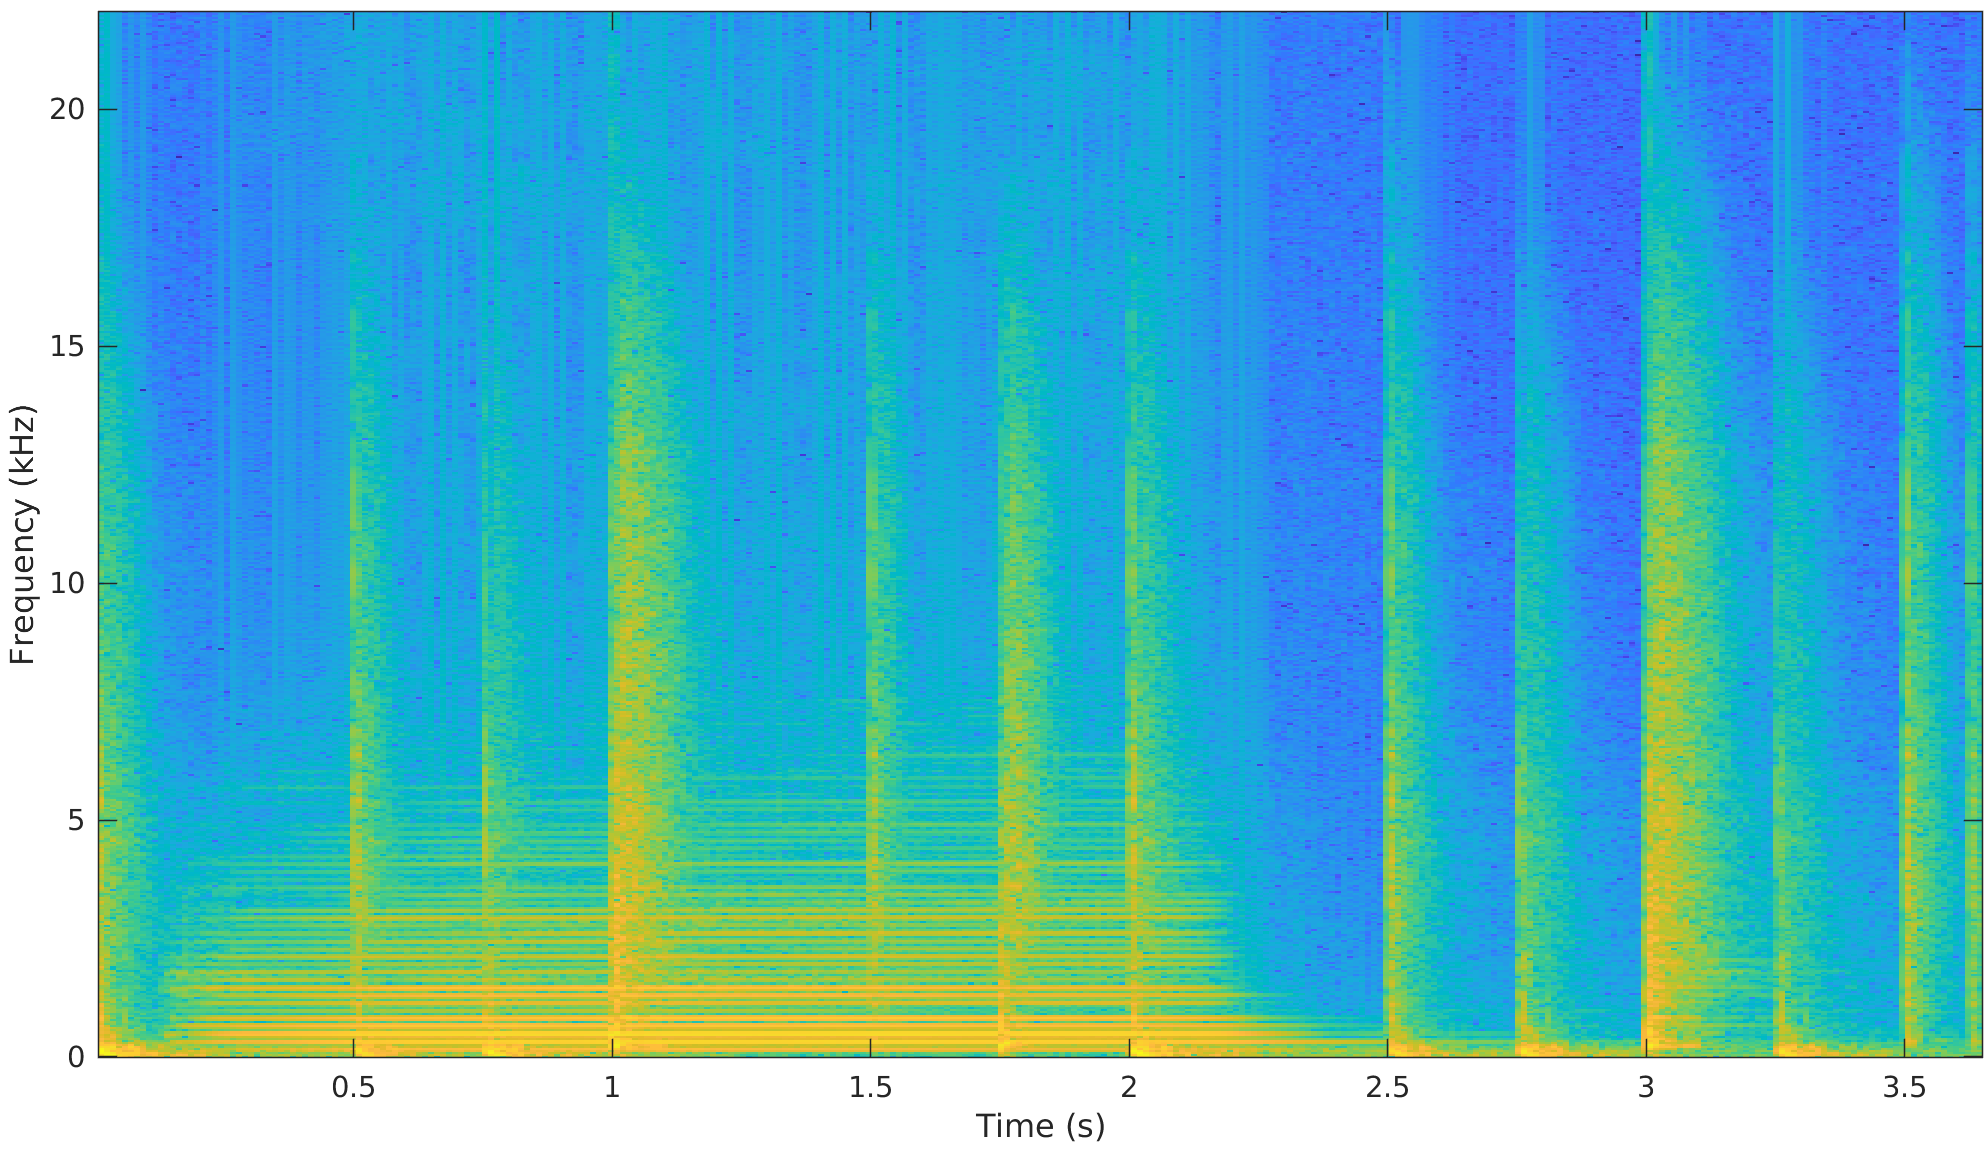
\includegraphics[width=6cm]{./mixedspecgram.png} }}
	\subfloat[Percussive separation]{{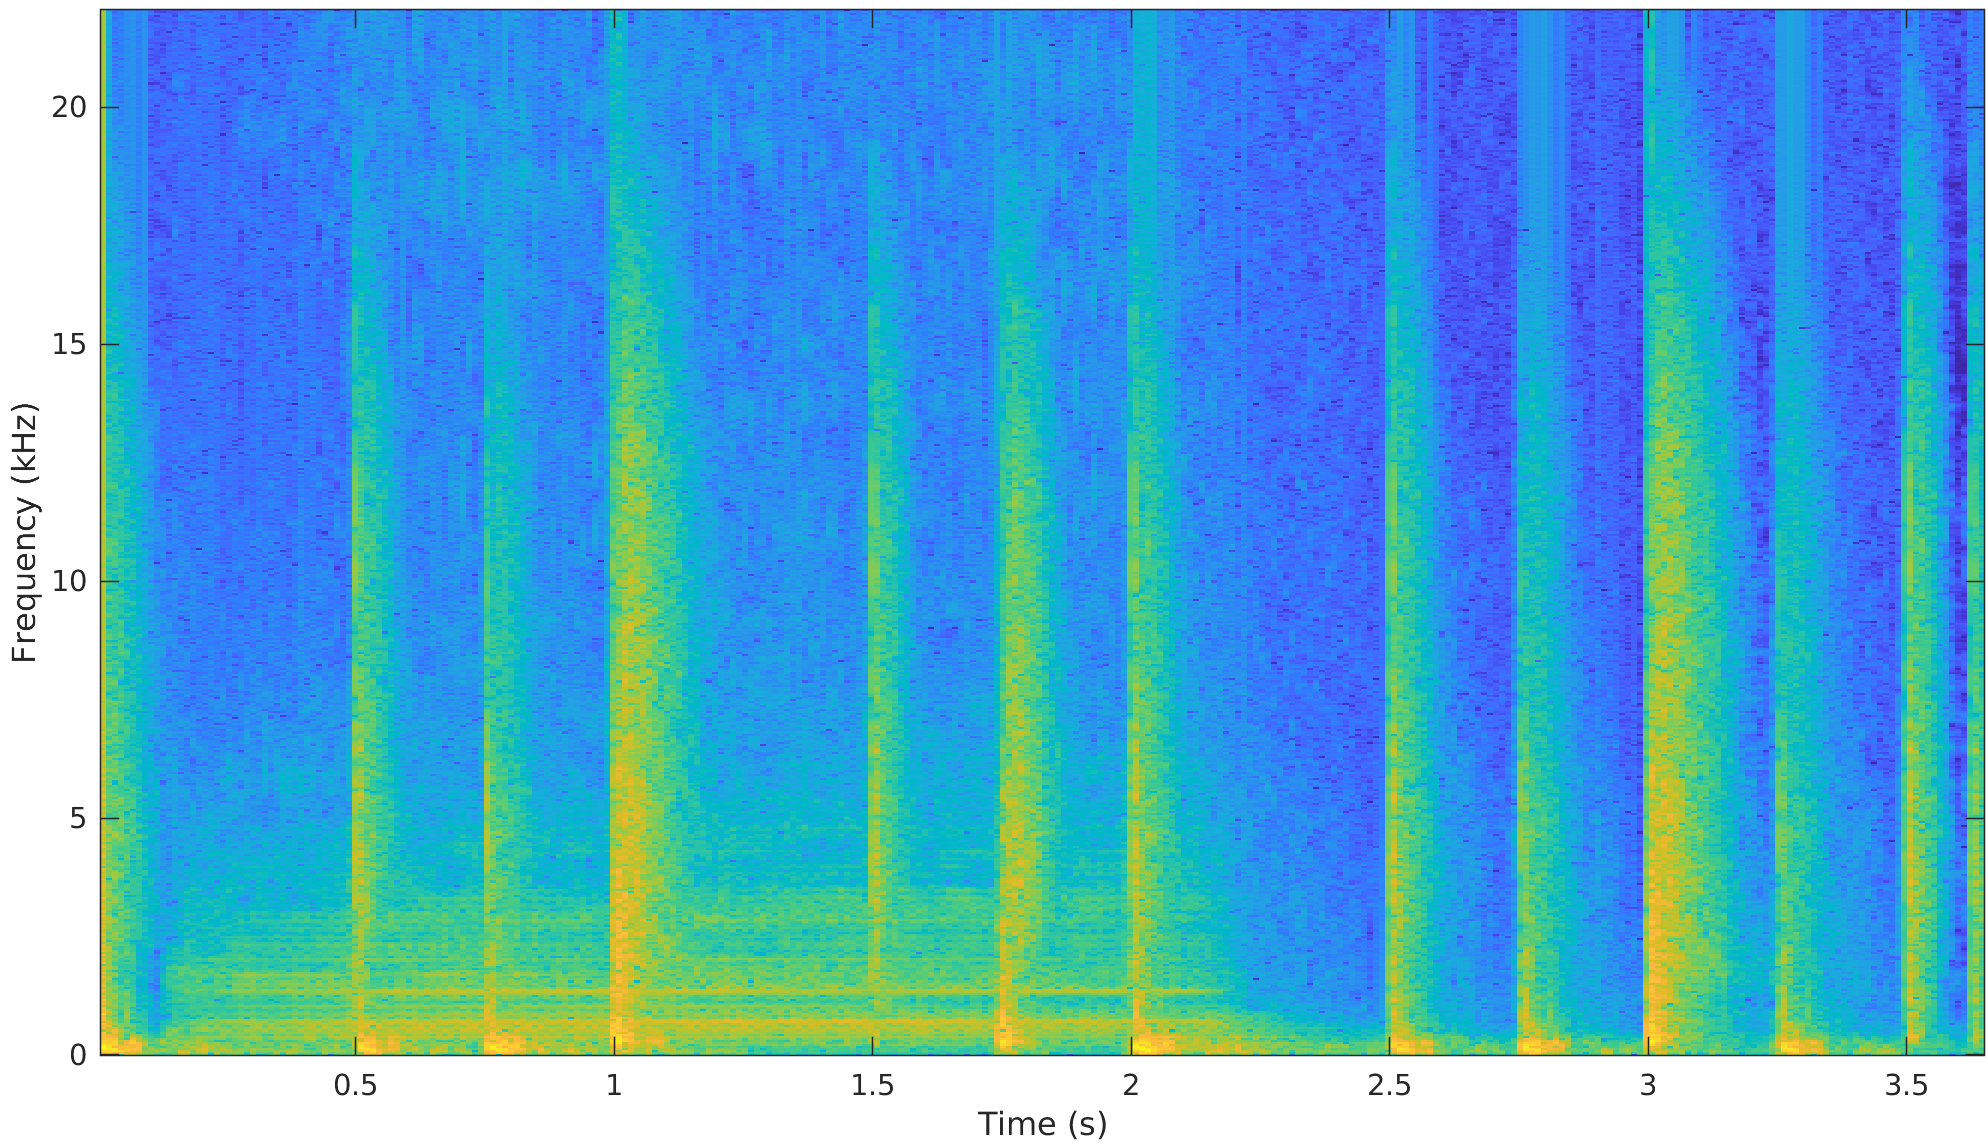
\includegraphics[width=6cm]{./perc_soft.png} }}
	\subfloat[Harmonic separation]{{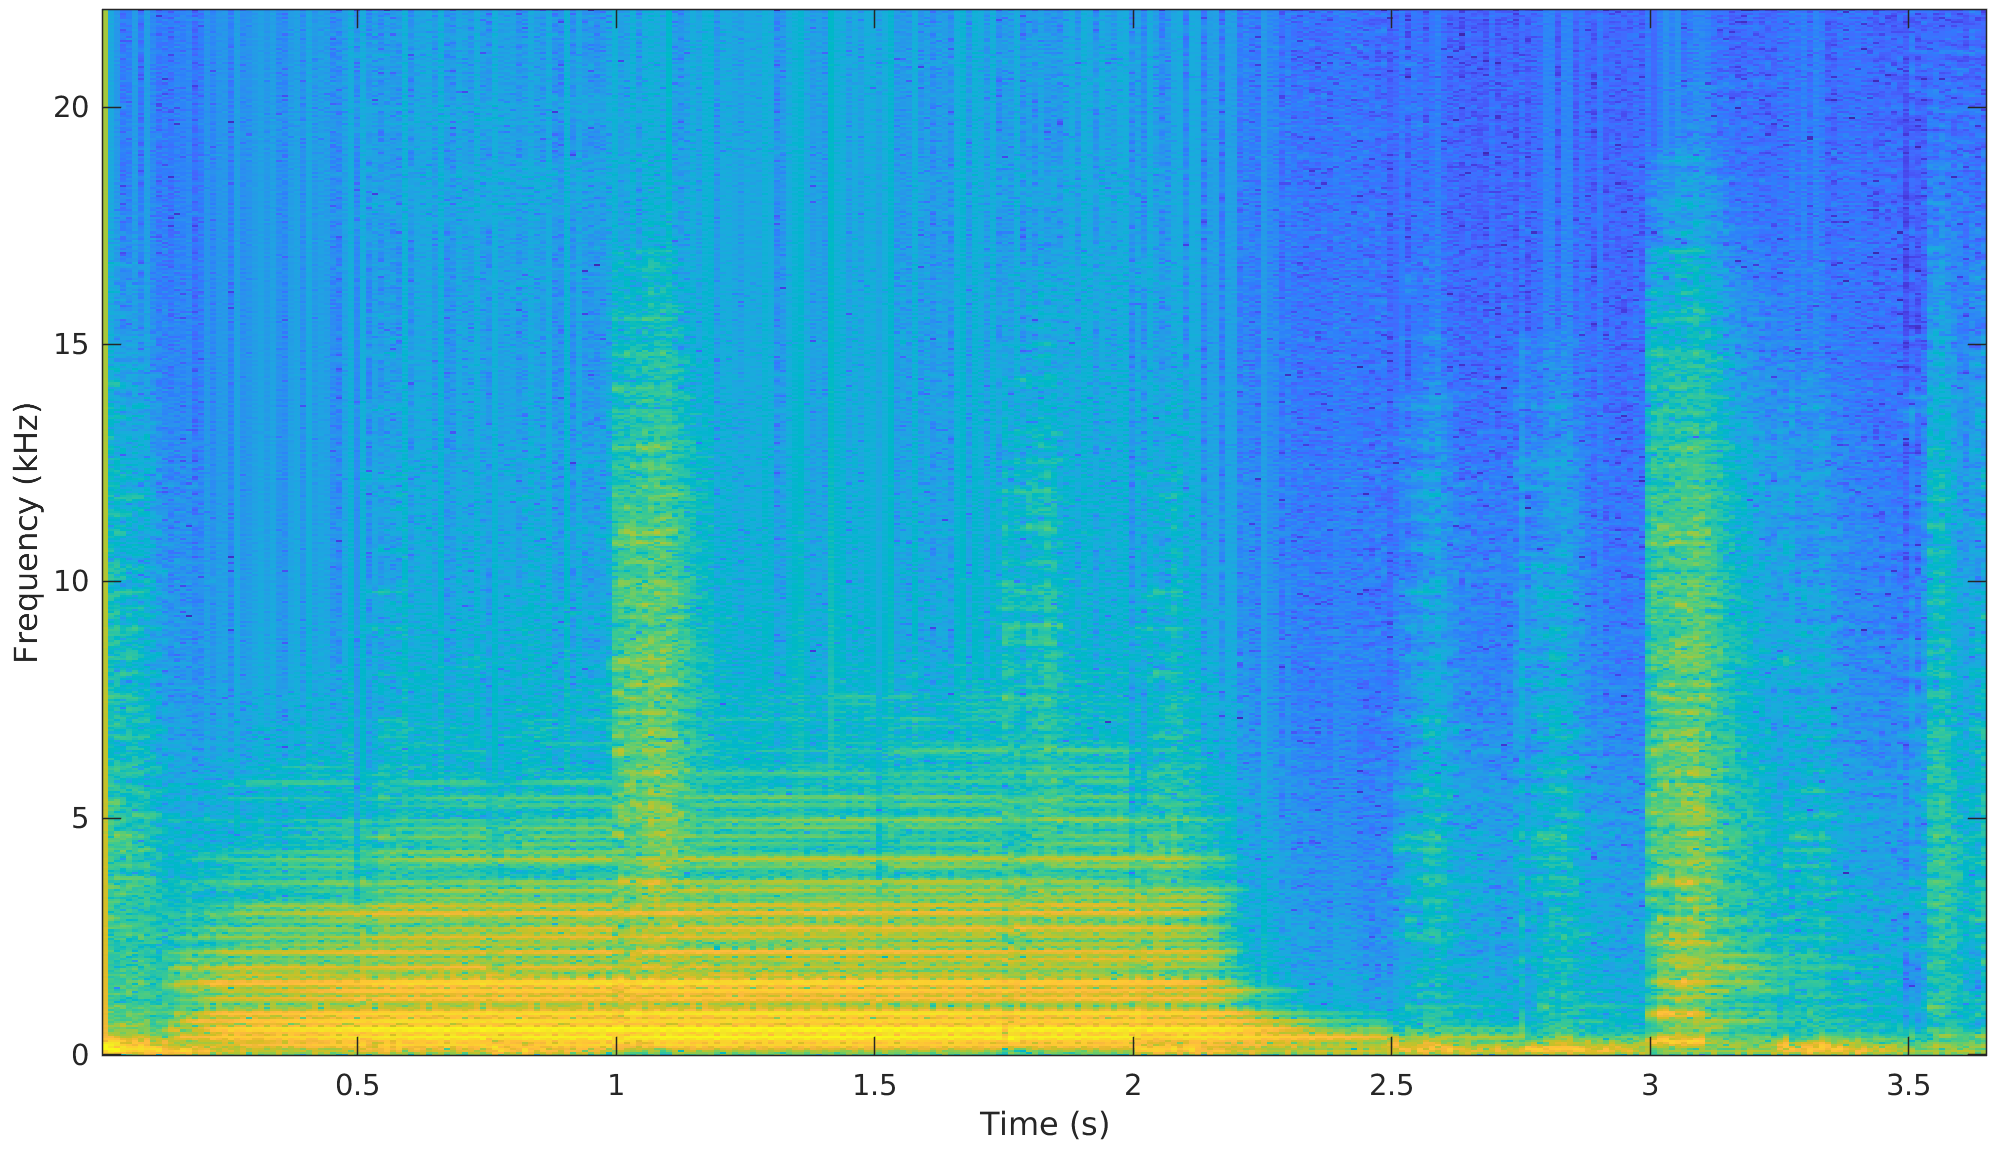
\includegraphics[width=6cm]{./harm_soft.png} }}
	\caption{Example of median-filtering HPSS}
	\label{fig:fitz1}
\end{figure}

\citet{driedger} replaced the soft mask with a binary/hard mask, and also introduced a two-pass variant. The first pass separates the harmonic component using an STFT with a large window size for high frequency resolution, followed by the second pass which separates the percussive component using an STFT with a small window size for high time resolution. \citet{fitzgerald2} created a similar iterative variant using soft masks. Additionally, they noted that when they replaced the small-window STFT with the constant-Q transform in the second pass, they obtained a separation of the human singing voice.

\begin{wrapfigure}{r}{8cm}
	\vspace{-1.0em}
	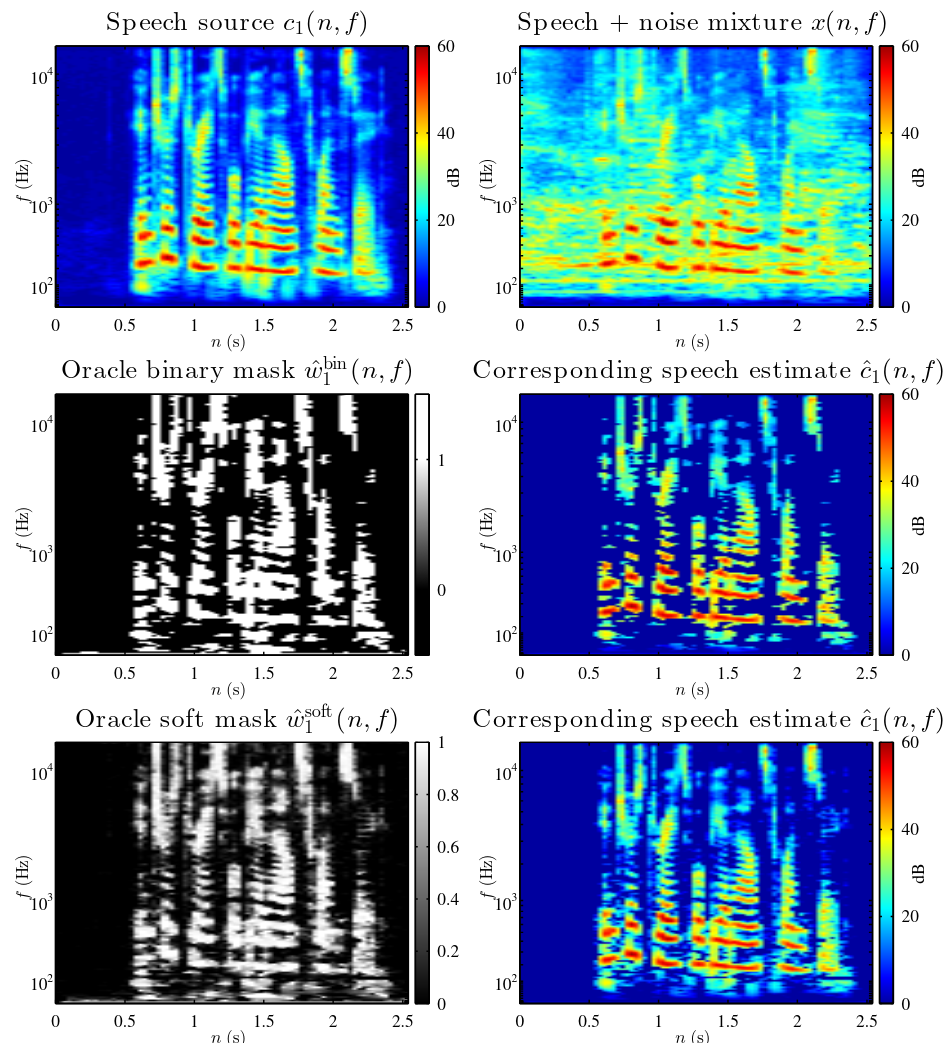
\includegraphics[width=8cm]{./maskdemo.png}
	\caption{Results of a soft and hard oracle mask applied for speech denoising}
	\label{fig:masks}
\end{wrapfigure}

\citet{masking} describe different time-frequency masking strategies in audio source separation. A time-frequency mask (or spectral mask, or masking filter), is a matrix of the same size as the complex STFT, by which the STFT is multiplied to mask/filter/suppress specific time-frequency tiles. A soft mask has real values $\in [0, 1]$, and a binary or hard mask has logical values, i.e. only 0 and 1. Soft masks generally produce higher quality sound, as shown in figure \ref{fig:masks}. The oracle mask is the ideal mask for a given signal -- to compute it, the target signal must be known. The soft mask used in \cite{fitzgerald1, fitzgerald2} is a Wiener filter, of the form:

\[ M = \frac{\text{target}^{2}}{\text{target}^{2} + \text{interference}^{2}} \]

The hard mask used in \cite{driedger} is of the form:

\[ M = \frac{\text{target}}{\text{interference}+\epsilon} \le \beta \]

, where $\beta$ is the separation factor. Note the inclusion of machine epsilon in the denominator, to avoid division by zero.

\subsection{TFJigsaw}

The next algorithm considered is the Time-Frequency Jigsaw Puzzle\cite{tfjigsaw}, which is implemented in the Large Time-Frequency Analysis toolbox \cite{ltfat, tfjigsaw2, tfjigsaw3}. Tonal/transient (or harmonic/percussive) separation is among one of the possible applications of TFJigsaw. The insight is similar to the multipass approach described previously -- in a TF representation with high frequency resolution, tonal sounds are well-represented, and in a TF representation with high time resolution, transient sounds are well-represented:

\begin{quote}
	[...] the starting point is to define the tonal layer of the signal as the ``component'' which admits a sparse expansion with respect to a Gabor frame with high frequency resolution (i.e. with a wide window), and the transient layer as the ``component'' which admits a sparse expansion with respect to a Gabor frame with high time resolution (i.e. a narrow window).
\end{quote}

\begin{figure}[ht]
	\centering
	\subfloat[Two lattices within a super-tile; the rectangular region is the super-tile, the ellipses represent the domains within which each TF atom's spectrogram exceeds some fixed threshold, and the dots represent their center (the TF sampling points)]{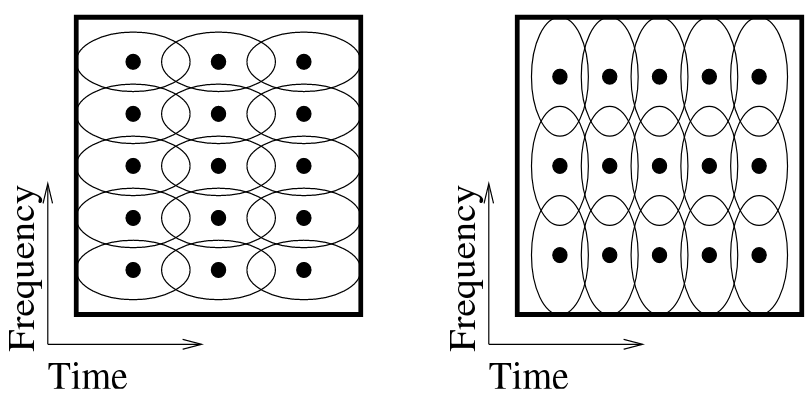
\includegraphics[height=4cm]{./tfjigsaw-supertiles.png}}
	\hspace{1em}
	\subfloat[$G^{0}$ and $G^{1}$ represent the analysis maps for the two Gabor frames, $\tilde{G}^{0}_{p}$ and $\tilde{G}^{1}_{p}$ represent the partial synthesis maps from the selected TF atoms, and $\mathcal{H}$ represents the calculation of entropy and corresponding decision]{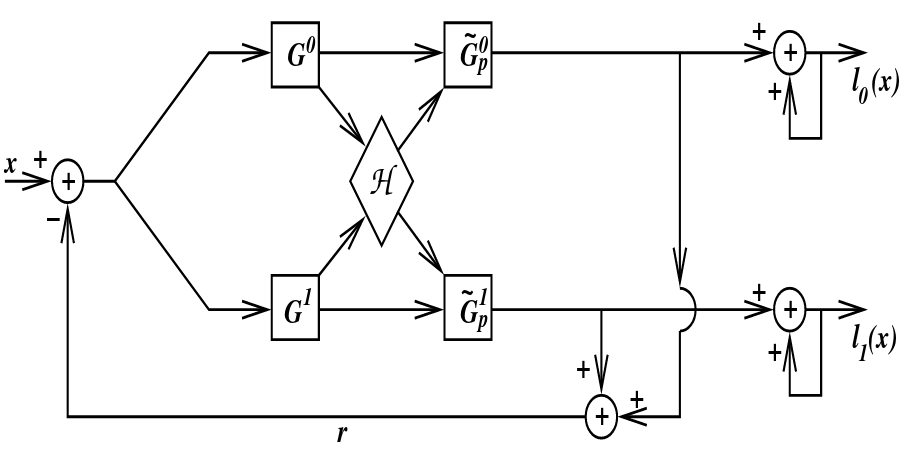
\includegraphics[height=4cm]{./tfjigsaw-entropycriterion.png}}
	\caption{\citet{tfjigsaw}'s illustrations of the TF Jigsaw Puzzle}
	\label{fig:supertiles}
\end{figure}

After creating two representations of the signal (one tonal with a large window Gabor frame, one transient with a small window Gabor frame), these are superimposed in a single time-frequency plane to create so-called ``super-tiles.'' The next task is to separate the components; within each super-tile, an entropy criterion chooses which tile (tonal or transient) is represented better and below a threshold, and subtracts these from the original signal. This is performed iteratively until the tonal and transient layers emerge. The super-tiles and entropy criterion are shown in figure \ref{fig:supertiles}, and the results are shown in figure \ref{fig:tfjigsawdemo}.

\begin{figure}[ht]
	\centering
	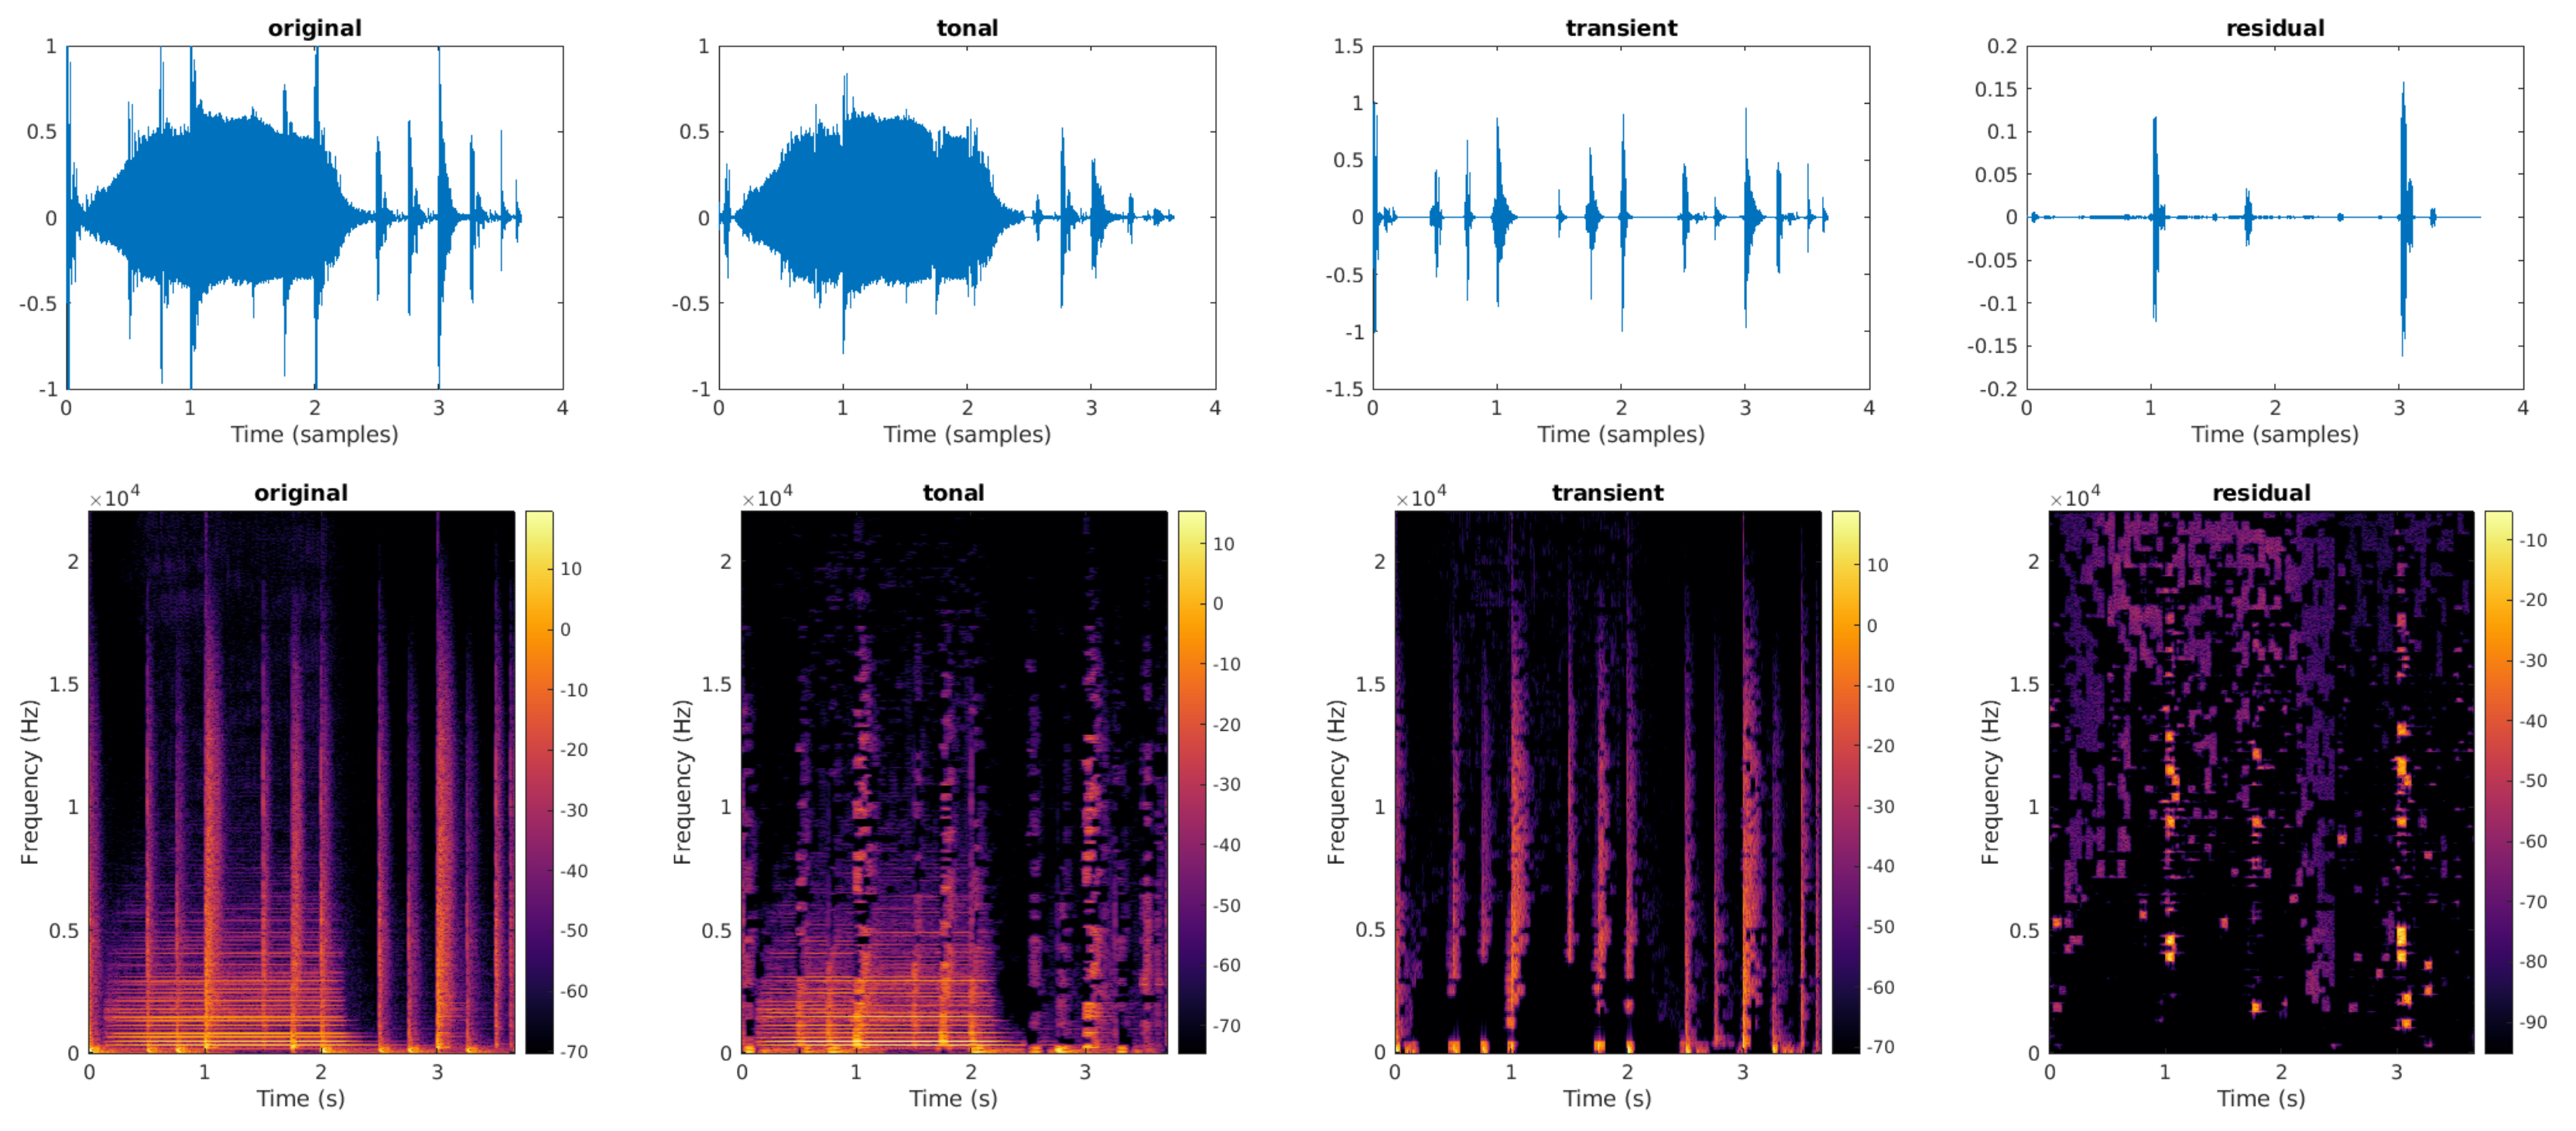
\includegraphics[width=16cm]{./tfjigsaw-sep-example.png}
	\caption{TFJigsawSep for tonal/transient separation}
	\label{fig:tfjigsawdemo}
\end{figure}

Note that the terms \textit{sparsity} and \textit{entropy} (w.r.t. TF analysis and audio signal representation) will be given a deeper treatment in section \ref{sec:theory}.

\subsection{WMDCTLasso}

The final algorithm for tonal/transient separation considered is referred to as ``WMDCTLasso.'' In LTFAT, its name is ``Audioshrink.''\cite{wmdct3}. The technique is described in a paper by \citet{wmdct}, and several demos on websites are available \cite{wmdct2, wmdct3}.

The WMDCTLasso algorithm performs a decomposition based on structured sparsity. It uses WMDCTs (Windowed Modified Discrete Cosine Transform) applied with two different time-frequency resolutions, by using a wide and narrow window -- with the wide window, the tonal sounds are well-represented, and with the narrow window, transient sounds are well-represented.

Next, a method called group lasso shrink is applied to separate the tonal and transient layers by exploiting their respective sparsity in each time-frequency representation. An example of a resulting decomposition of jazz music is shown in figure \ref{fig:wmdctex}.

\begin{figure}[ht]
	\centering
	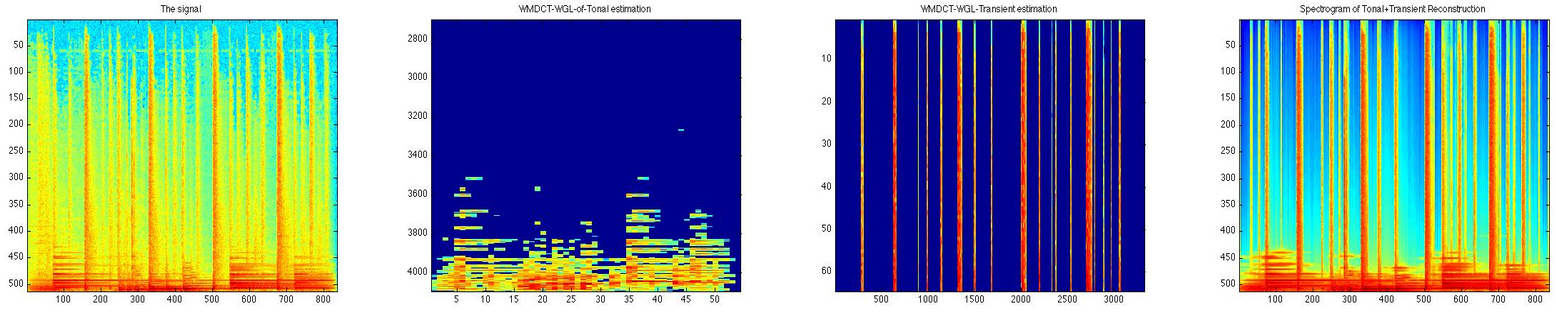
\includegraphics[width=16cm]{./wmdctjazz.png}
	\caption{WMDCTLasso for tonal/transient separation in jazz music}
	\label{fig:wmdctex}
\end{figure}

The term \textit{sparsity} is encountered again. In place of using an entropy criterion like in TFJigsaw, instead a technique called lasso shrinkage (or specifically, the group lasso variant) is used. The goal is the same -- to determine which part of the signal is best represented by the wide-window time-frequency representation, which is likely the tonal component, and similar for the case of the transient components and narrow window.

%%%%%%%%%%%%%%
% THEORY     %
%%%%%%%%%%%%%%
\section{Theory}
\label{sec:theory}

In all of the presented algorithms, there is at least one, but more commonly two, Gabor dictionaries built from the input signal, using different Gabor atoms. The STFT and CQT are well-known Gabor systems, while TFJigsaw and WMDCTLasso build their own custom Gabor dictionaries using the low-level frame functions available in LTFAT. This requires a general overview of what Gabor analysis and Gabor dictionaries are, and a demonstration of a signal represented with each of the time-frequency representations used by the different algorithms.

Second, the terms sparse signal representation and entropy are encountered in TFJigsaw and WMDCTLasso, which will be explained further. It will also be shown that the median filter used in the simpler HPSS algorithms, by isolating transients as vertical lines and tonal sounds as horizontal lines, is a form of exploiting sparsity in the time-frequency plane.

\subsection{\textbf{\textcolor{red}{TODO }}Tonal and transient sounds}

\subsection{\textbf{\textcolor{red}{TODO }}Gabor dictionaries and time-frequency representations}

\subsection{\textbf{\textcolor{red}{TODO }}Sparsity, entropy, and matching pursuit}

%%%%%%%%%%%%%%%
% METHODOLOGY %
%%%%%%%%%%%%%%%
\section{Methodology}
\label{sec:methodology}

\subsection{Objective measures}

The SigSep (\href{https://sigsep.github.io/}{https://sigsep.github.io/}) community, borrowing from the methodology of Signal Separation Evaluation Campaign (SISEC), uses the BSS (Blind Source Separation) Eval \cite{bss} objective measure for separation quality. The authors of BSS released an improved version that matches better with subjective human evaluations, which they called the PEASS (Perceptual Evaluation methods for Audio Source Separation) Toolkit \cite{peass}, based on PEMO-Q \cite{pemoq}. The PEASS Toolkit for MATLAB \cite{peassmatlab} conveniently includes all 3 measures: PEASS, PEMO-Q, and BSS. Each of these consist of 4 metrics:

\begin{tight_itemize}
\item
	\textbf{Target:} measure of desired sound in the separation. TPS (Target Perceptual Score) in PEASS, ISR (source Image to Spatial distortion Ratio) in BSS, qTarget in PEMO-Q.
\item
	\textbf{Interference:} measure of undesired sounds in the separation. IPS (Interference Perceptual Score) in PEASS, SIR (Signal to Interference Ratio) in BSS, qInterf in PEMO-Q.
\item
	\textbf{Artifacts:} measure of artifacts in the separation. APS (Artifact Perceptual Score) in PEASS, SAR (Signal to Artifacts Ratio) in SAR, qArtif in PEMO-Q.
\item
	\textbf{Global:} a global score for the previous three. In PEASS, this is OPS (Overall Perceptual Score). In BSS, this is SDR (Signal to Distortion Ratio). In PEMO-Q, this is qGlobal.
\end{tight_itemize}

\citet{beassvpeass} make the recommendation to use PEASS for music separation evaluation, noting the importance of perception in music applications. They also recommend to evaluate algorithms based on their separate target, interference, and artifact scores, noting that the global measure of OPS (for PEASS) and SDR (for BSS) have an uncertain relation to the three constituent scores. The choice in this paper is to use the three individual metrics from the PEASS:
\begin{tight_enumerate}
	\item
		\textbf{TPS} (Target Perceptual Score)
	\item
		\textbf{APS} (Artifact Perceptual Score)
	\item
		\textbf{IPS} (Interference Perceptual Score)
\end{tight_enumerate}

\subsection{Evaluated music}

The most popular music stem dataset used by SISEC and SigSep is the MUSDB18 dataset \cite{musdb18} (or the HQ, high-quality, equivalent \cite{musdb18-hq}). MUSDB18-HQ contains stems (.wav files per component/instrument, e.g., drum.wav, vocal.wav, bass.wav) from a collection of permissively licensed music, specifically intended for recording, mastering, mixing (and in this case, ``de-mixing'', or source separation) research. 

A limited subset of MUSDB18-HQ was evaluated, or 5 total minutes of music, consisting of 4 segments of 15 seconds duration taken from 5 separate tracks. One data set was prepared for harmonic/percussive separation evaluation (vocals omitted from the mix), and one data set for harmonic/percussive/vocal evaluation (vocals are present). The evaluation was limited to 5 minutes of music since the PEASS measure is computationally expensive.

The songs in the MUSDB18-HQ dataset are split into train and test sets. Since the final comparison of this paper will consider a neural network model which was trained on MUSDB18, the evaluation data is taken from the test set -- if we took it from the training set, the neural network could overfit and overperform.

\subsection{Evaluation format}

Due to the large number of algorithms and configurations that will be evaluated, introducing them all at the same time will be overwhelming, and will make it difficult to form conclusions. The proposed format will be like an ``elimination tournament,'' similar to sports tournaments. Starting from the simplest one-pass algorithm for harmonic/percussive source separation, we can perform evaluations to form intermediate conclusions:

\begin{tight_itemize}
\item
	Is the STFT or CQT better for harmonic/percussive source separation
\item
	Which window size of STFT (out of 128, 256, 1024, 2048, 4096, 16384), or which bins-per-octave of CQT (12, 24, 48, 96), performs best
\item
	Which of soft or hard masking performs best
\end{tight_itemize} 

From these, we can move on to two-pass variants, by using the conclusions from the previous evaluation. Next, we can evaluate the TF jigsaw and WMDCT group lasso methods with different configurations. After the harmonic/percussive evaluations are done, we can introduce vocal separation, and repeat. The initial evaluations will be described in the following section, \ref{sec:elim}.

The final goal is to combine the best performers to create optimal ``hybrid'' algorithms for each task: HPSS and harmonic/percussive/vocal separation. The construction of the hybrid algorithms will be shown in detail in section \ref{sec:hybrids}. At the last stage, the optimal hybrids will be compared to Open-Unmix \cite{umx}. Open-Unmix is a deep-learning-based music source separation system which achieves near state-of-the-art results. It is fully open-source, and was intended to be a reference and benchmark in the field of signal separation.

\subsection{Python/MATLAB testbench}

The language chosen to implement the algorithms was MATLAB. It is an obvious choice since it has access to LTFAT, the PEASS Toolkit, many other signal processing tools (e.g., Wavelet Toolbox), and is in general a natural choice for prototyping digital signal processing algorithms. On the other hand, certain tasks for the project are more easily accomplished with Python. One example is in the preparation of the datasets, which requires traversing directories of stem files to produce mix and reference harmonic/percussive/vocal files. Also, Python would be a good choice for data visualization and result aggregation, to be able to use numpy\cite{numpy}, pandas\cite{pandas}, matplotlib\cite{matplotlib}, and seaborn\cite{seaborn}. The solution is to employ both languages wherever appropriate, and use the file system and JSON as universal interchanges:
\begin{tight_enumerate}
\item
	The Python script for data preparation scans the stem directories of MUSDB18-HQ, creates test wav files with a prefix indicating a unique sequence number, and wav files for each of the mix, harmonic, percussive, and vocal components
\item
	The MATLAB testbench script finds all mix files, executes the separation algorithms being tested on each, and writes the separated component outputs to a directory with the algorithm name, e.g., ``1pass-hpss-f-cqt-24,'' for easy identification.
\item
	The MATLAB testbench script calculates the median PEASS scores across all of the testcases, and prints a JSON-encoded string containing the algorithm names and scores.
\item
	The Python result analysis script takes the JSON string as an input, and produces heatmaps for reporting and visualization.
\end{tight_enumerate}

One final issue is that Open-Unmix, the deep learning solution chosen as a reference, is implemented for Python with pytorch\cite{pytorch}. The solution was to write a MATLAB shim script for Open-Unmix, which uses the `system' command in MATLAB to run Open-Unmix using the operating system. In this way, every algorithm could be executed by the MATLAB testbench.

%%%%%%%%%%%%%%%%%%%%%%%%%%
% Evaluations %
%%%%%%%%%%%%%%%%%%%%%%%%%%
\section{Algorithm evaluations}
\label{sec:elim}

\textbf{N.B.:} as a shorthand, STFT with window size X will be referred to as STFT-X, and CQT with bins-per-octave X will be referred to as CQT-X. For example, CQT-96 is a CQT with 96 bins-per-octave, and STFT-2048 is an STFT with window size 2048.

\subsection{Harmonic/percussive source separation}

The first task is harmonic/percussive source separation. The mixtures are combined from the instrument stems (excluding vocals). The evaluation is performed on 5 minutes of music from MUSDB18-HQ, as was mentioned. The results are displayed as colored heatmaps, where green is the best result and red is the worst. This enables a quick visual verification of the best performers.

\subsubsection{Median-filtering with STFT/CQT masking}
\label{subsec:mfilthpss}

We can consider two generalized frameworks for harmonic/percussive (and optionally vocal) source separation with masking and median filtering of either the STFT and CQT, considering the one-pass and two-pass variants separately. In both cases, we can substitute different window sizes of STFT, or the CQT with different bins per octave, to test the effects. The block diagram of the system under test is shown in figure \ref{fig:fitz2}, and the algorithms are described in listing \ref{lst:pseudocodes}.

\begin{figure}[ht]
	\centering
	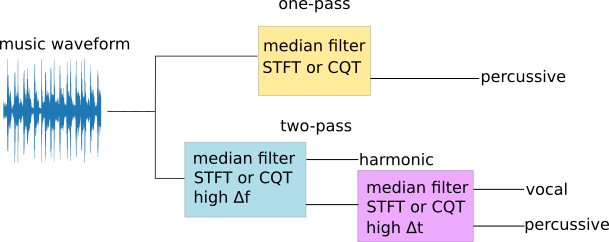
\includegraphics[width=10cm]{./medianfiltdiagram.png}
	\caption{A general framework for median filtering music separation}
	\label{fig:fitz2}
\end{figure}

The first and original median-filtering HPSS algorithm with soft masks was introduced by \citet{fitzgerald1}. The modification introduced by \citet{driedger} uses hard masks (the same paper contains the two-pass variant, which will be discussed later).

\begin{figure}[h]
  \centering
 \begin{minipage}{0.48\textwidth}
  \centering
\begin{minted}[numbersep=\mintednumbersep,linenos,mathescape=true,breaklines,frame=single,escapeinside=||]{text}
|$s = \text{mixed audio}$|
|$\hat{S} = \text{STFT}(s)\text{\textbf{ or CQT}}$|
|$S = \text{abs}(\hat{S})$|
|$H = \text{medianfilter}(S, l_{H}, \text{axis}=2)$|
|$P = \text{medianfilter}(S, l_{P}, \text{axis}=1)$|
|$\text{\textbf{soft} } M_{H} = \frac{H^{p}}{H^{p} + P^{p}}, M_{P} = \frac{P^{p}}{H^{p} + P^{p}}$|
|$\text{\textbf{hard} } M_{H} = \frac{H}{P + \epsilon} \ge \beta, M_{P} = \frac{P}{H + \epsilon} > \beta$|
|$\hat{H} = \hat{S} \cdot M_{H}$|
|$\hat{P} = \hat{S} \cdot M_{P}$|
|$h = \text{ISTFT}(\hat{H})\text{\textbf{ or ICQT}}$|
|$p = \text{ISTFT}(\hat{P})\text{\textbf{  or ICQT}}$|
\end{minted}
 \end{minipage}
\hspace{0.02\textwidth}
 \begin{minipage}{0.48\textwidth}
  \centering
\begin{minted}[numbersep=\mintednumbersep,linenos,mathescape=true,breaklines,frame=single,escapeinside=||]{text}
|$s = \text{mixed audio}$|
|$\hat{S1} = \text{STFT}(s, \text{window}=4096)\text{\textbf{ or CQT}}$|
|$ \text{apply one-pass algorithm to get } \hat{H1}, \hat{P1} $|
|$\text{\textbf{final harmonic} } h1 = \text{ISTFT}(\hat{H1})\text{\textbf{ or ICQT}}$|
|$p1 = \text{ISTFT}(\hat{P1})\text{\textbf{ or ICQT}}$|
|$\hat{S2} = \text{STFT}(p1, \text{window}=256)\text{\textbf{ or CQT}}$|
|$ \text{apply one-pass algorithm to get } \hat{H2}, \hat{P2} $|
|$h2 = \text{ISTFT}(\hat{H2})\text{\textbf{ or ICQT}}$|
|$\text{\textbf{final percussive} } p1 = \text{ISTFT}(\hat{P2})\text{\textbf{ or ICQT}}$|
\end{minted}
 \end{minipage}
  \captionof{listing}{1- and 2-pass median-filtering HPSS algorithms}
  \label{lst:pseudocodes}
\end{figure}

Some parameters are fixed in the evaluation, since they're not relevant to time-frequency resolution. Median filter lengths of $l_{H} = l_{P} = 17$ were used for the STFT, and $l_{H} = 17, l_{P} = 7$ for the CQT (as suggested in \cite{fitzgerald1, fitzgerald2}). The power for the soft masking was set to $p = 2$, and the separation factor for the hard masking was set to $\beta = 2$ (as suggested in \cite{fitzgerald1, driedger}). The results can be seen in figures \ref{fig:round1soft} and \ref{fig:round1hard}. The naming scheme for the tested configurations is described in table \ref{table:round1hpss}.

\begin{table}[ht]
	\centering
\begin{tabular}{ |l|l|c|c| }
	 \hline
	  Name & Configuration \\
	 \hline
	 \hline
	 x1pass\_hpss\_f\_\{128-16384\} & 1-pass Fitzgerald (soft mask) with STFT of size 128-16384 \\
	 \hline
	 x1pass\_hpss\_f\_cqt\_\{12-96\} & 1-pass Fitzgerald (soft mask) with CQT of bins-per-octave 12-96 \\
	 \hline
	 x1pass\_hpss\_d\_\{128-16384\} & 1-pass Driedger (hard mask) with STFT of size 128-16384 \\
	 \hline
	 x1pass\_hpss\_d\_cqt\_\{12-96\} & 1-pass Driedger (hard mask) with CQT of bins-per-octave 12-96 \\
	 \hline
\end{tabular}
	\caption{One-pass HPSS configuration naming scheme}
	\label{table:round1hpss}
\end{table}

With soft masking, using CQT-96 achieves the best score in both the harmonic and percussive separation's target, and is the best performer from all variants in percussive separation. In the harmonic separation, the evaluated STFT configurations showed better interference and worse artifacts compared to the CQT configurations. With hard masking, all of the evaluations showed poor target and artifact scores. This is consistent with the quality of soft versus hard time-frequency masking mentioned in the masking overview \cite{masking} in the introduction. CQT-96 outperforms all the STFTs for harmonic separation in the hard masking algorithm. The STFT-2048 performs the best at percussive separation.

CQT-96 demonstrates good results for both harmonic and percussive separation with soft masks, indicating it has both desired qualities: high frequency resolution, originally achieved with a large-window STFT, and high time resolution, originally achieved with a small-window STFT. This makes it a good choice for one-pass harmonic/percussive source separation.

\begin{figure}[ht]
	\centering
	\makebox[\textwidth]{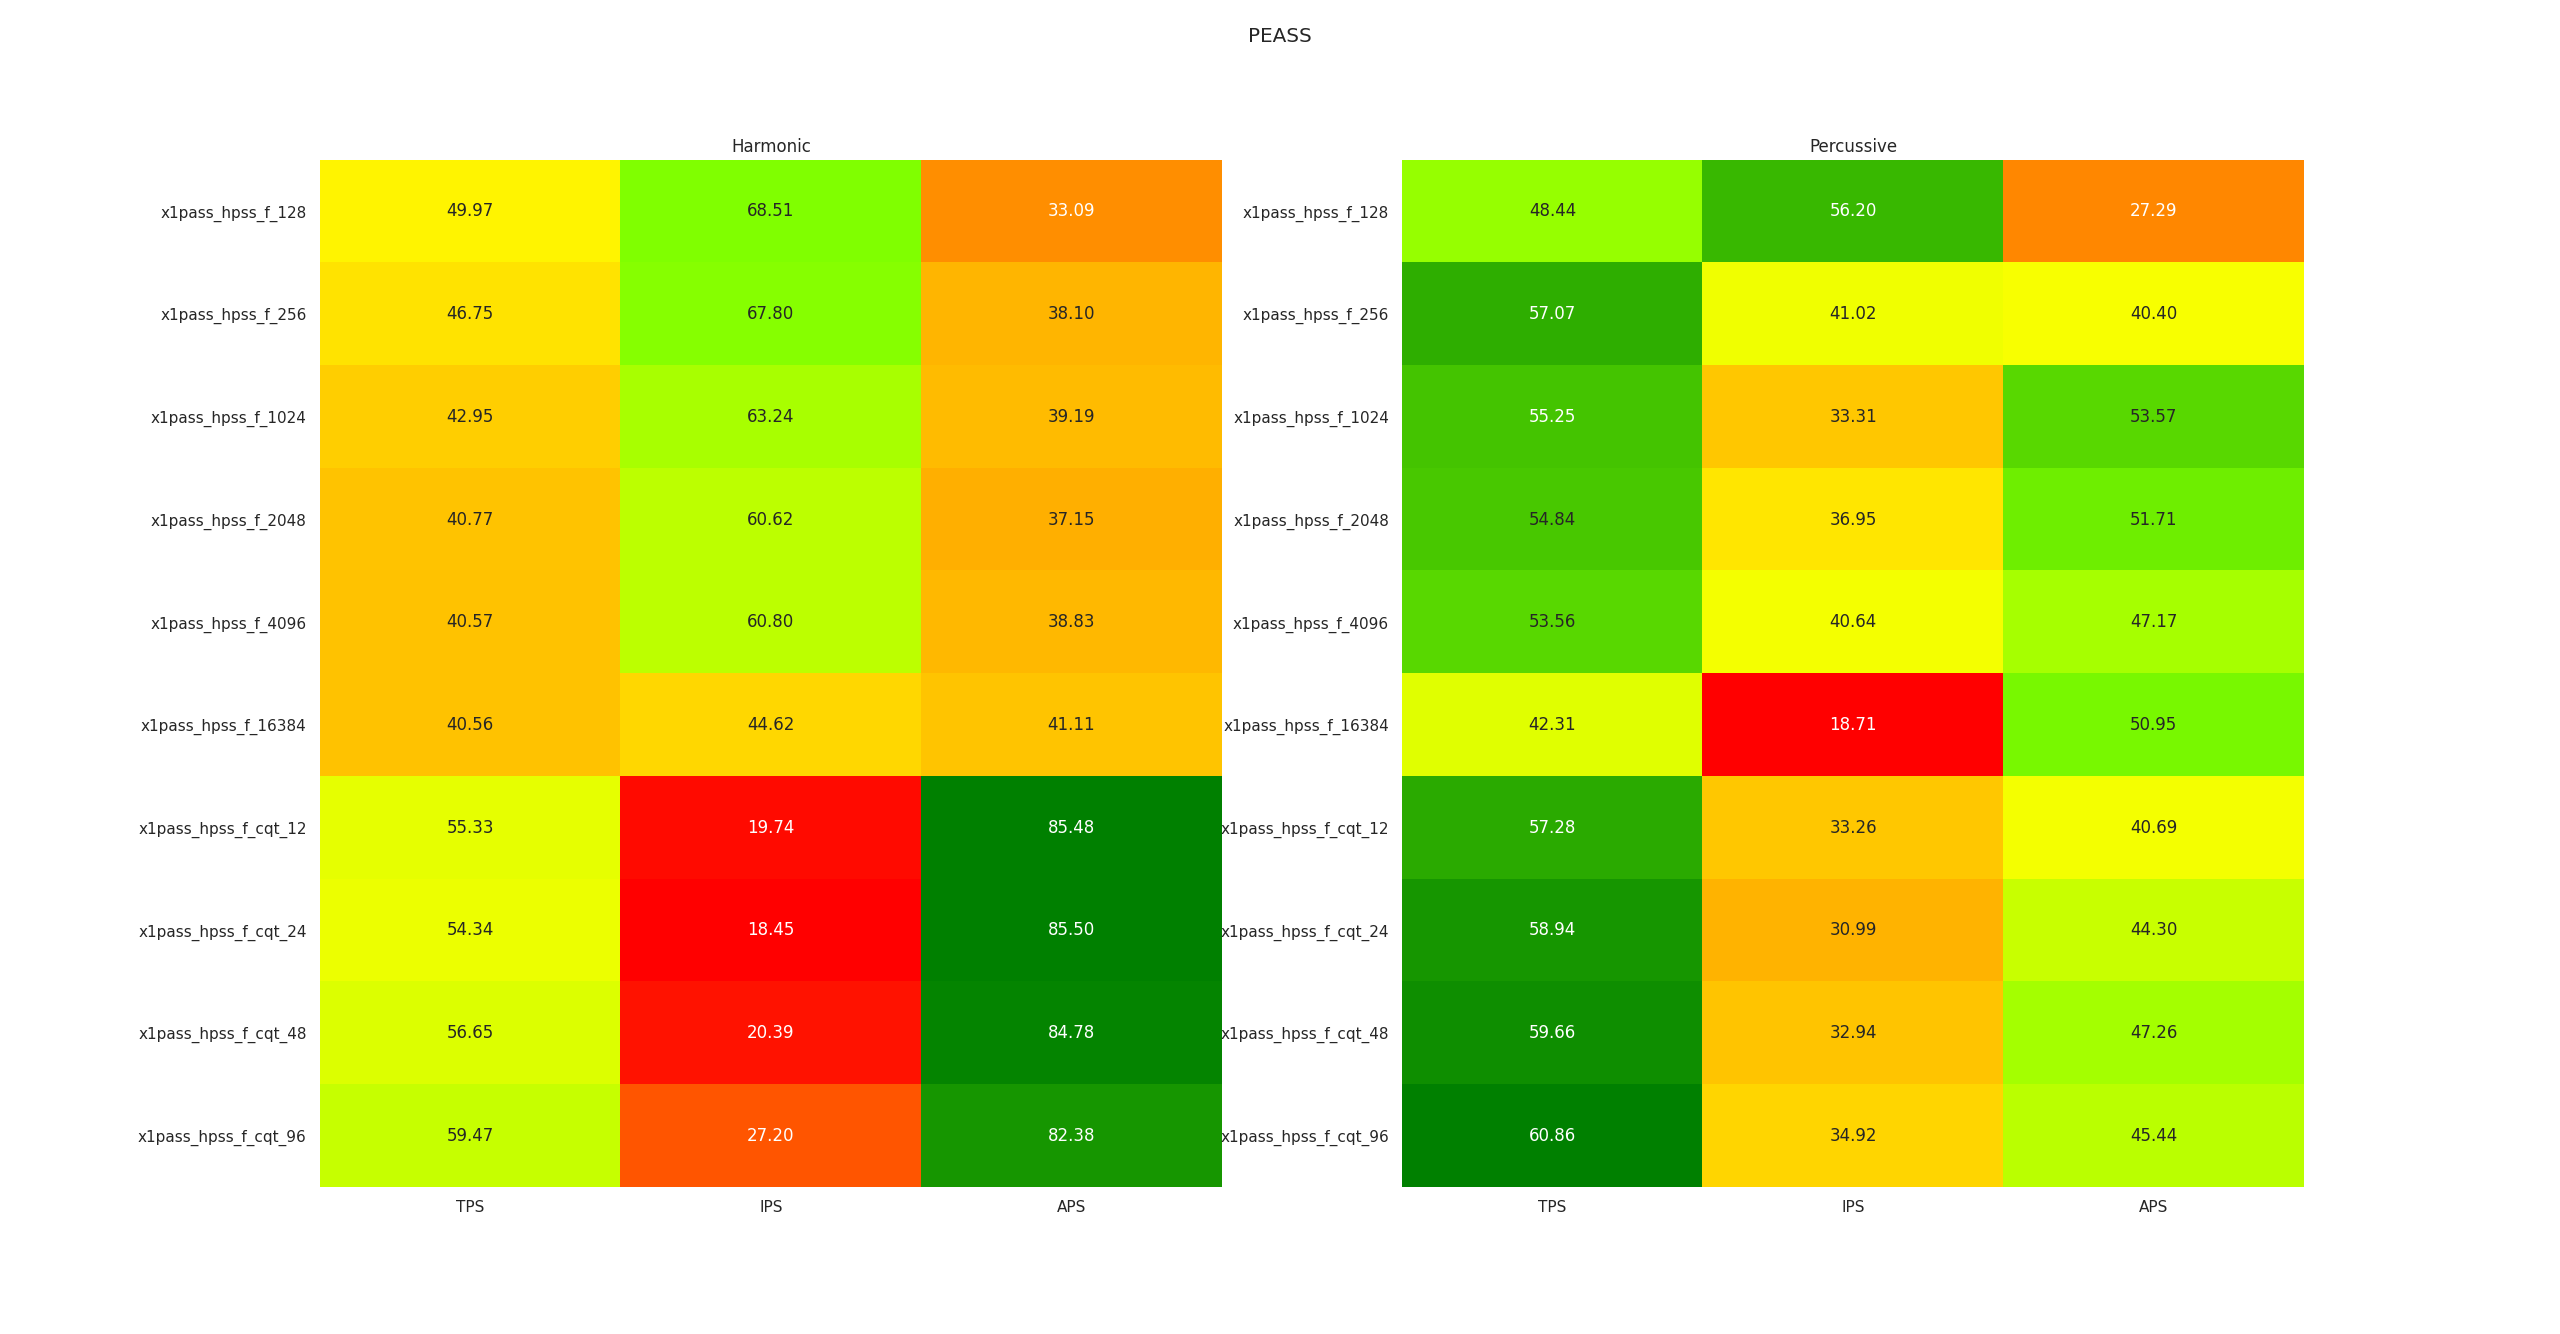
\includegraphics[width=16cm]{../evaluation/heatmaps/1pass_Fitzgerald_PEASS_abbrev.png}}
	\caption{One-pass soft-masking PEASS results}
	\label{fig:round1soft}
\end{figure}

\begin{figure}[ht]
	\centering
	\makebox[\textwidth]{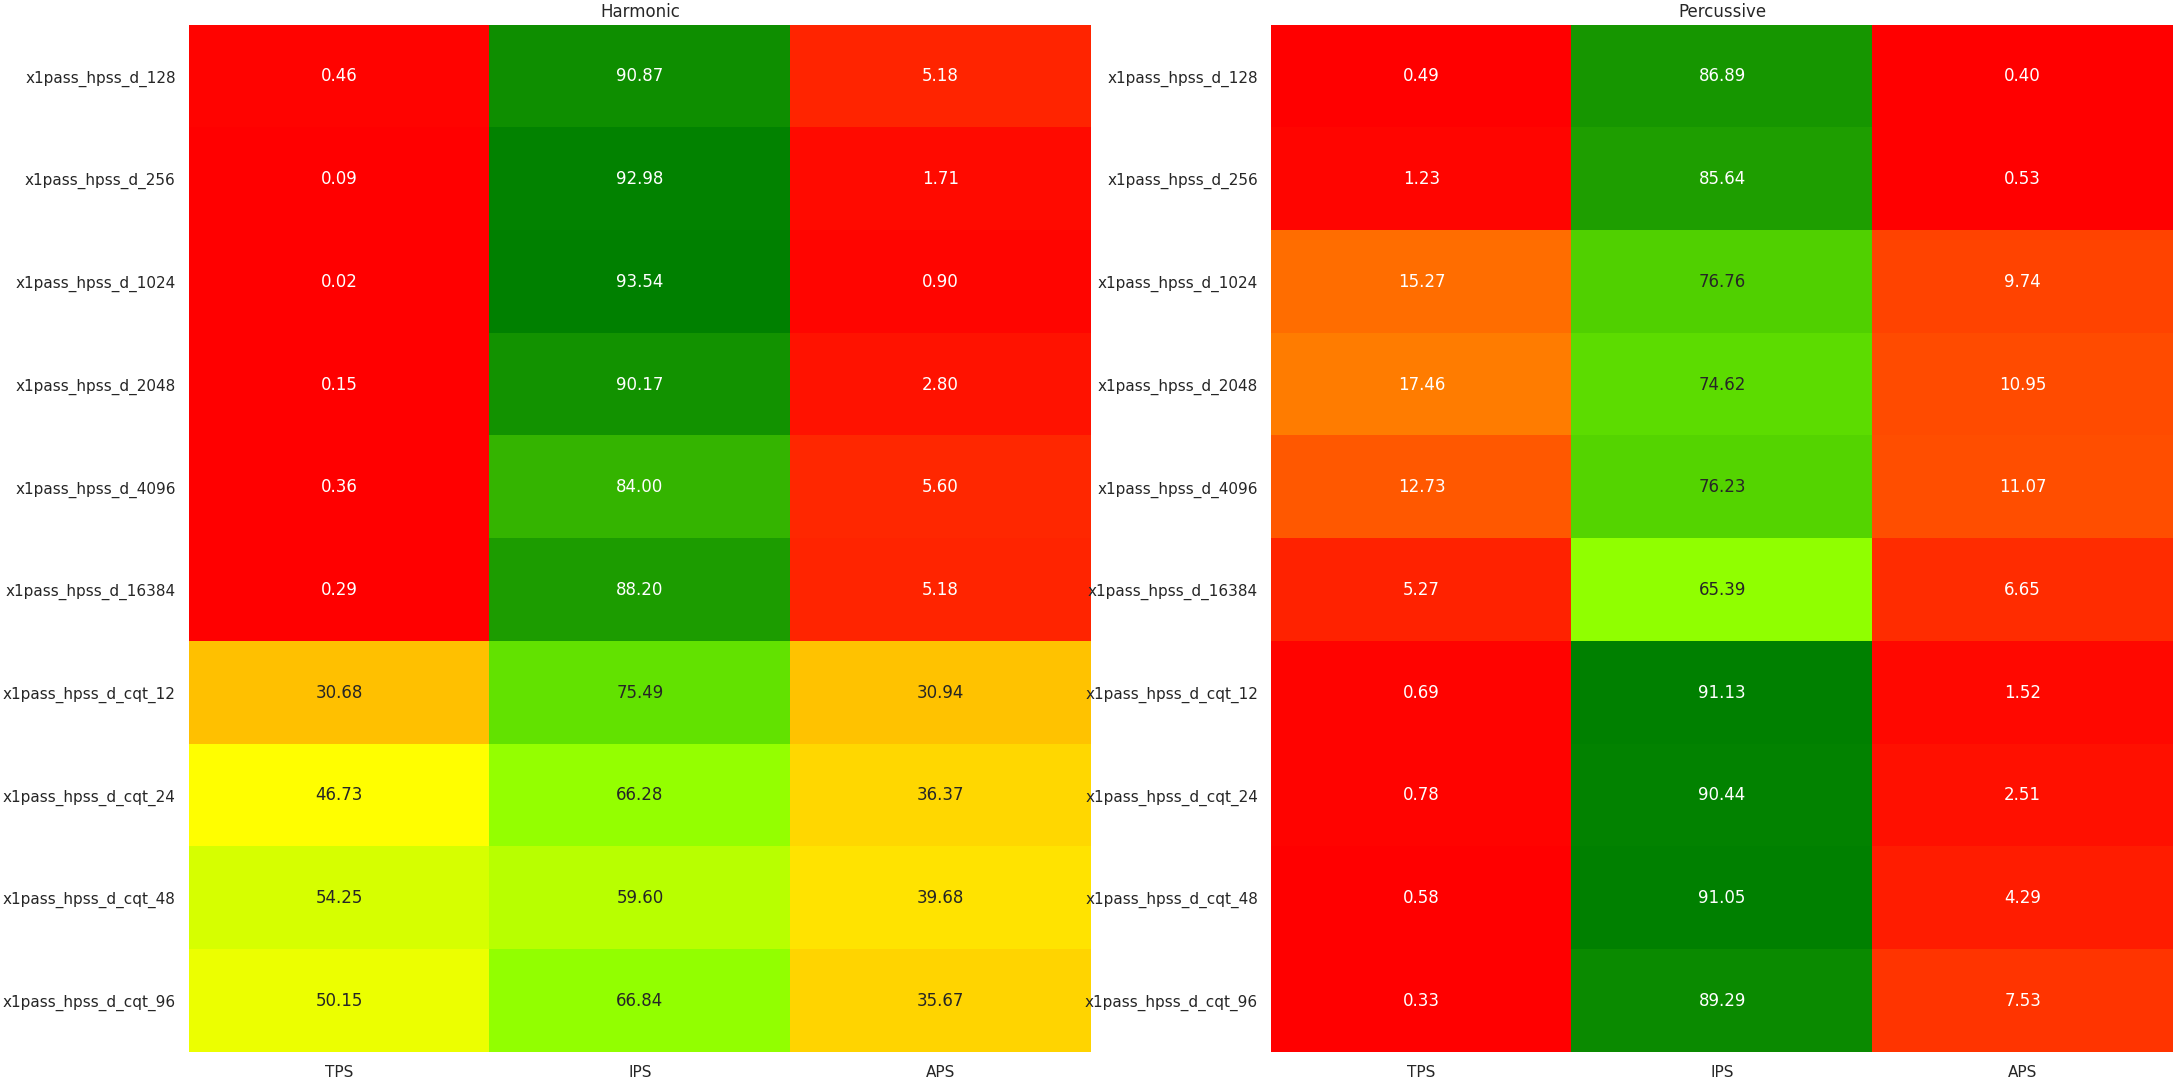
\includegraphics[width=16cm]{../evaluation/heatmaps/1pass_Driedger_PEASS_abbrev.png}}
	\caption{One-pass hard-masking PEASS results}
	\label{fig:round1hard}
\end{figure}

\subsubsection{Two-pass algorithms with STFT/CQT masking}

\citet{driedger}'s iterative algorithm is presented for harmonic/percussive source separation. The algorithm is shown in listing \ref{lst:pseudocodes}. The conclusions from the previous round of testing are used to prepare 3 variants of two-pass hard masking HPSS:
\begin{tight_enumerate}
	\item
		The first variant, ``id'' (Iterative Driedger), uses an STFT-16384 in the first pass, and an STFT-2048 in the second pass (the best performing STFT configurations for harmonic and percussive separation, respectively).
	\item
		The second variant, ``id\_cqt1'' uses a CQT-96 in the first pass for the harmonic separation (top harmonic performer), and STFT-2048 (top percussive performer) in the second pass.
	\item
		The third variant, ``id\_default,'' is the default with the exact settings (STFT-4096 for harmonic, STFT-256 for percussive) from the paper \cite{driedger}.
\end{tight_enumerate}

The results in figure \ref{fig:round2hard} show that the CQT-96/STFT-2048 algorithm performs the best. By the PEASS evaluation, the target and artifact scores for the CQT-96/STFT-2048 variant are better, at the expense of a slightly lower interference score.

\begin{figure}[ht]
	\centering
	\makebox[\textwidth]{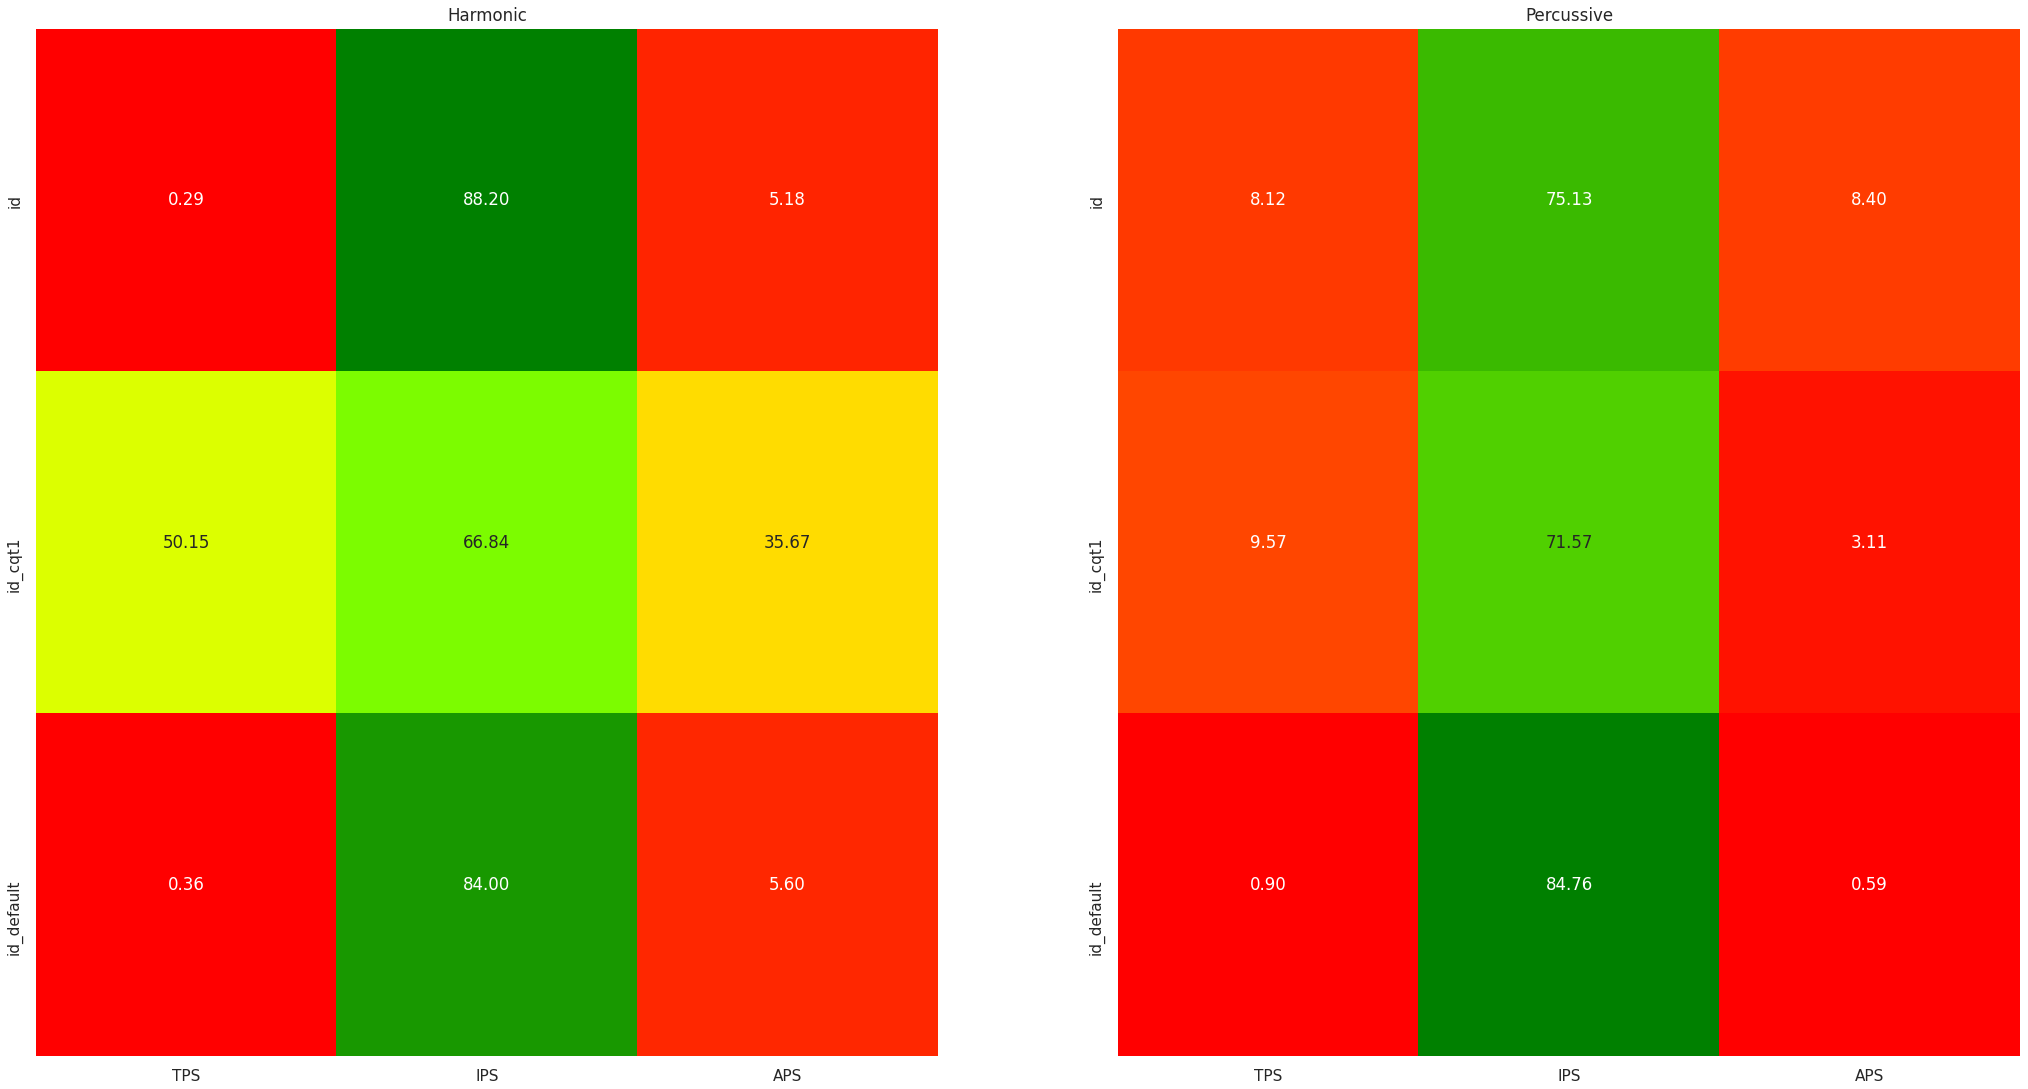
\includegraphics[width=14cm]{../evaluation/heatmaps/2pass_Driedger_PEASS_abbrev.png}}
	\caption{Two-pass hard-masking PEASS results}
	\label{fig:round2hard}
\end{figure}

\subsubsection{TFJigsaw}

An algorithm considered which uses a custom time-frequency analysis is the Time-Frequency Jigsaw Puzzle \cite{tfjigsaw}, implemented in LTFAT \cite{tfjigsaw2}. The implementation was adapted directly from the LTFAT demo \cite{tfjigsaw3}. Similar to the STFT or CQT algorithms above, the tfjigsawsep function in LTFAT allows for configuring the window size of the Gabor systems used for the tonal and transient components, which can be considered analogous to the two-pass methods seen above. The default settings are a Hann window of size 4096 for the tonal system and 256 for the transient system. The TFJigsaw algorithm is described in listing \ref{lst:tfjigsaw}.

\begin{figure}[h]
  \centering
  \centering
\begin{minted}[numbersep=\mintednumbersep,linenos,mathescape=true,breaklines,frame=single,escapeinside=||]{text}
|$f = \text{mixed audio}$|
|$a,M,\text{winsize},b\{1,2\} = \text{Gabor systems 1 and 2 configuration}$|
|$[\text{ref}1, \text{ref}2] = \text{generate estimate of random white noise entropy within supertile}$|
|$[\text{tau}1, \text{tau}2] = [\text{ref}1 \cdot r1, \text{ref}2 \cdot r2]$|
|$c1 = \text{DGTReal}(f, \text{winsize}1, a1, M1)\qquad\text{\textbf{Discrete Gabor Transform}}$|
|$c2 = \text{DGTReal}(f, \text{winsize}2, a2, M2)$|
|$f1 = \text{frequency supertile location, Gabor system 1}$|
|$f2 = \text{frequency supertile location, Gabor system 2}$|
|$t1 = \text{time supertile location, Gabor system 1}$|
|$t2 = \text{time supertile location, Gabor system 2}$|
|$[c1, c2] = \text{decision}(c1,c2,f1,f2,t1,t2,\text{tau}1,\text{tau}2)$|
|$f_{\text{tonal}} = \text{IDGTReal}(c1)\qquad\qquad\text{\textbf{Inverse discrete Gabor Transform}}$|
|$f_{\text{transient}} = \text{IDGTReal}(c2)$|
\end{minted}
  \captionof{listing}{TFJigsaw tonal/transient separation algorithm}
  \label{lst:tfjigsaw}
\end{figure}

The \Verb#decision# function uses R{\'e}nyi entropy to decide whether a signal is more random than random white noise represented within a supertile, and sets those coefficients to zero. For example, a transient sound will have a high entropy, or randomness, in the tonal Gabor system -- worse than white noise -- so it can be set to zero, creating a tonal separation (and vice-versa for transient separation). A consequence of using random white noise (in line 3 of the code listing) is that TFJigsawsep is non-deterministic. That is, you can run TFJigsaw separation with the same input signal and the same parameters, and get back a different result due to the different random white noise generated for the entropy comparison.

The parameters of Jigsaw Sep are as follows: $v2$ uses version 2 of the algorithm, $p$ is the proportion of the time-frequency supertile relative to the step sizes, $r1$ is the significance level of the tonal layer compared to white noise, and $r2$ is the same for the transient layer. General recommendations are $r2 > r1$, $r2 \approx 1.05$ for good percussion, $v2 = true$ for good tonal, $p = \text{small}$ for music separation. A variety of parameters were tested, shown in table \ref{table:round2jigsaw}.

\begin{table}[ht]
	\centering
\begin{tabular}{ |l|l|l|l|l|l|l|c|c|c|c|c|c|c| }
	 \hline
	  Name & p & r1 & r2 & v2 & winsize1 & winsize2 \\
	 \hline
	 \hline
	 tfjigsaw-1 & 2 & 0.88 & 1.05 & false & 4096 & 256 \\
	 \hline
	 tfjigsaw-2 & 2 & 0.88 & 1.05 & true & 4096 & 256 \\
	 \hline
	 tfjigsaw-3 & 4 & 0.88 & 1.05 & false & 4096 & 256 \\
	 \hline
	 tfjigsaw-4 & 2 & 0.88 & 1.03 & false & 4096 & 256 \\
	 \hline
	 tfjigsaw-5 & 2 & 0.85 & 1.05 & false & 4096 & 256 \\
	 \hline
	 tfjigsaw-6 & 2 & 0.88 & 0.89 & false & 4096 & 256 \\
	 \hline
	 tfjigsaw-7 & 2 & 0.85 & 1.05 & true & 4096 & 256 \\
	 \hline
	 tfjigsaw-8 & 5 & 0.85 & 1.05 & true & 4096 & 256 \\
	 \hline
	 tfjigsaw-9 & 9 & 0.85 & 1.05 & true & 4096 & 256 \\
	 \hline
	 tfjigsaw-10 & 2 & 0.88 & 1.03 & false & 16384 & 4096 \\
	 \hline
	 tfjigsaw-11 & 2 & 0.88 & 1.03 & false & 8192 & 2048 \\
	 \hline
	 tfjigsaw-12 & 2 & 0.85 & 1.05 & true & 16384 & 4096 \\
	 \hline
	 tfjigsaw-13 & 2 & 0.85 & 1.05 & false & 16384 & 4096 \\
	 \hline
	 tfjigsaw-14 & 2 & 0.88 & 1.05 & false & 16384 & 256 \\
	 \hline
	 tfjigsaw-15 & 2 & 0.88 & 1.05 & false & 16384 & 2048 \\
	 \hline
	 tfjigsaw-16 & 2 & 0.88 & 1.05 & false & 16384 & 1024 \\
	 \hline
	 tfjigsaw-17 & 2 & 0.88 & 1.05 & false & 8192 & 512 \\
	 \hline
\end{tabular}
	\caption{TFJigsaw configurations}
	\label{table:round2jigsaw}
\end{table}

From the tested configurations in figure \ref{fig:jigsaw}, we can see that in fact, the harmonic separation of configuration \Verb#tfjigsaw-1# achieves excellent results for target and artifacts -- it does not have the highest interference score, but this is usually a tradeoff, with better interference resulting from more aggressive removal, which results in more artifacts. In a subjective listening test, \Verb#tfjigsaw-1# sounds the best. On the other hand, good parameters could not be found for percussive separation scores for the TFJigsaw, which almost all suffered from a low artifact score (i.e., suffered from a presence of artifacts). This doesn't necessarily mean that TFJigsaw  is bad at percussive separation -- further study might be required to explore why this is the case, and how the results can be improved.

\begin{figure}[ht]
	\centering
	\makebox[\textwidth]{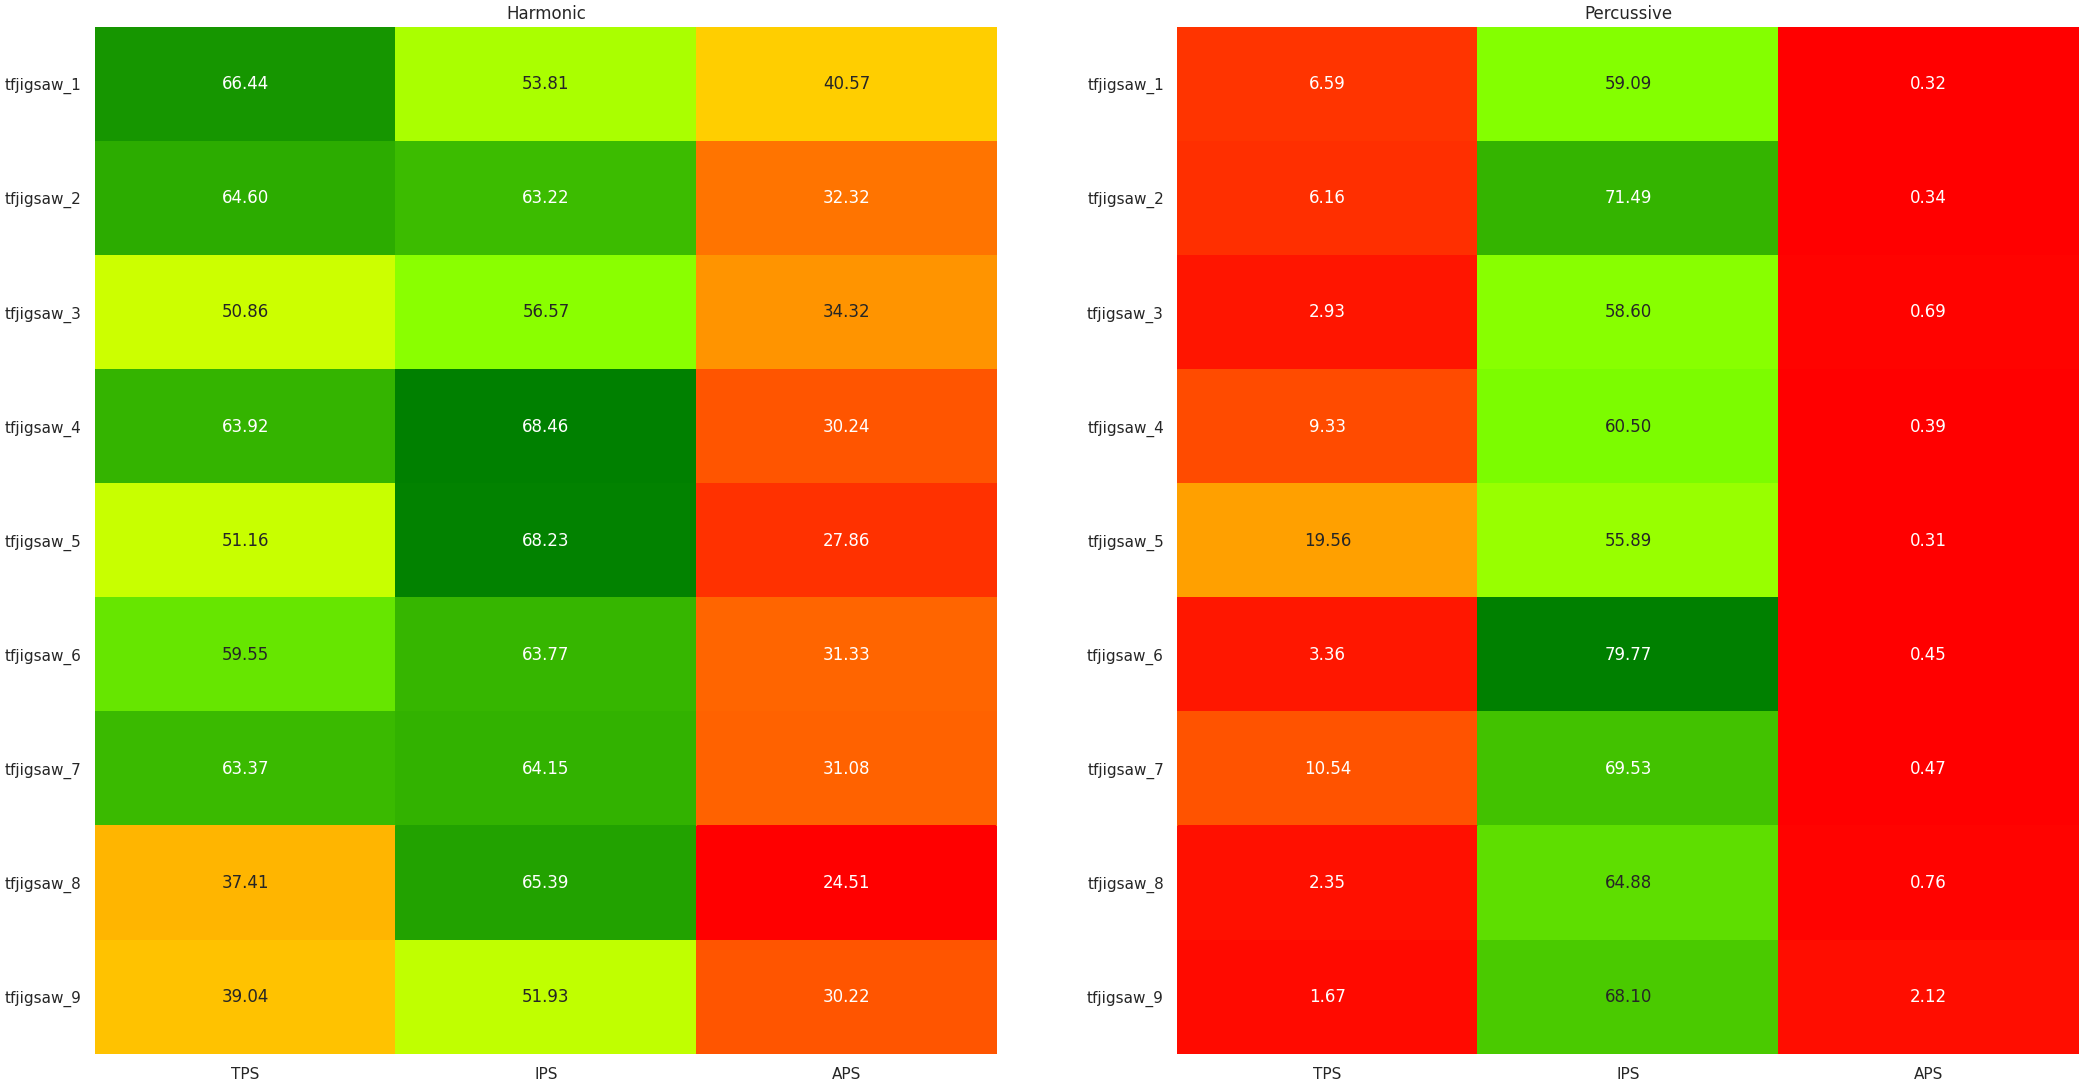
\includegraphics[width=16cm]{../evaluation/heatmaps/Jigsaw_PEASS_abbrev.png}}
	\makebox[\textwidth]{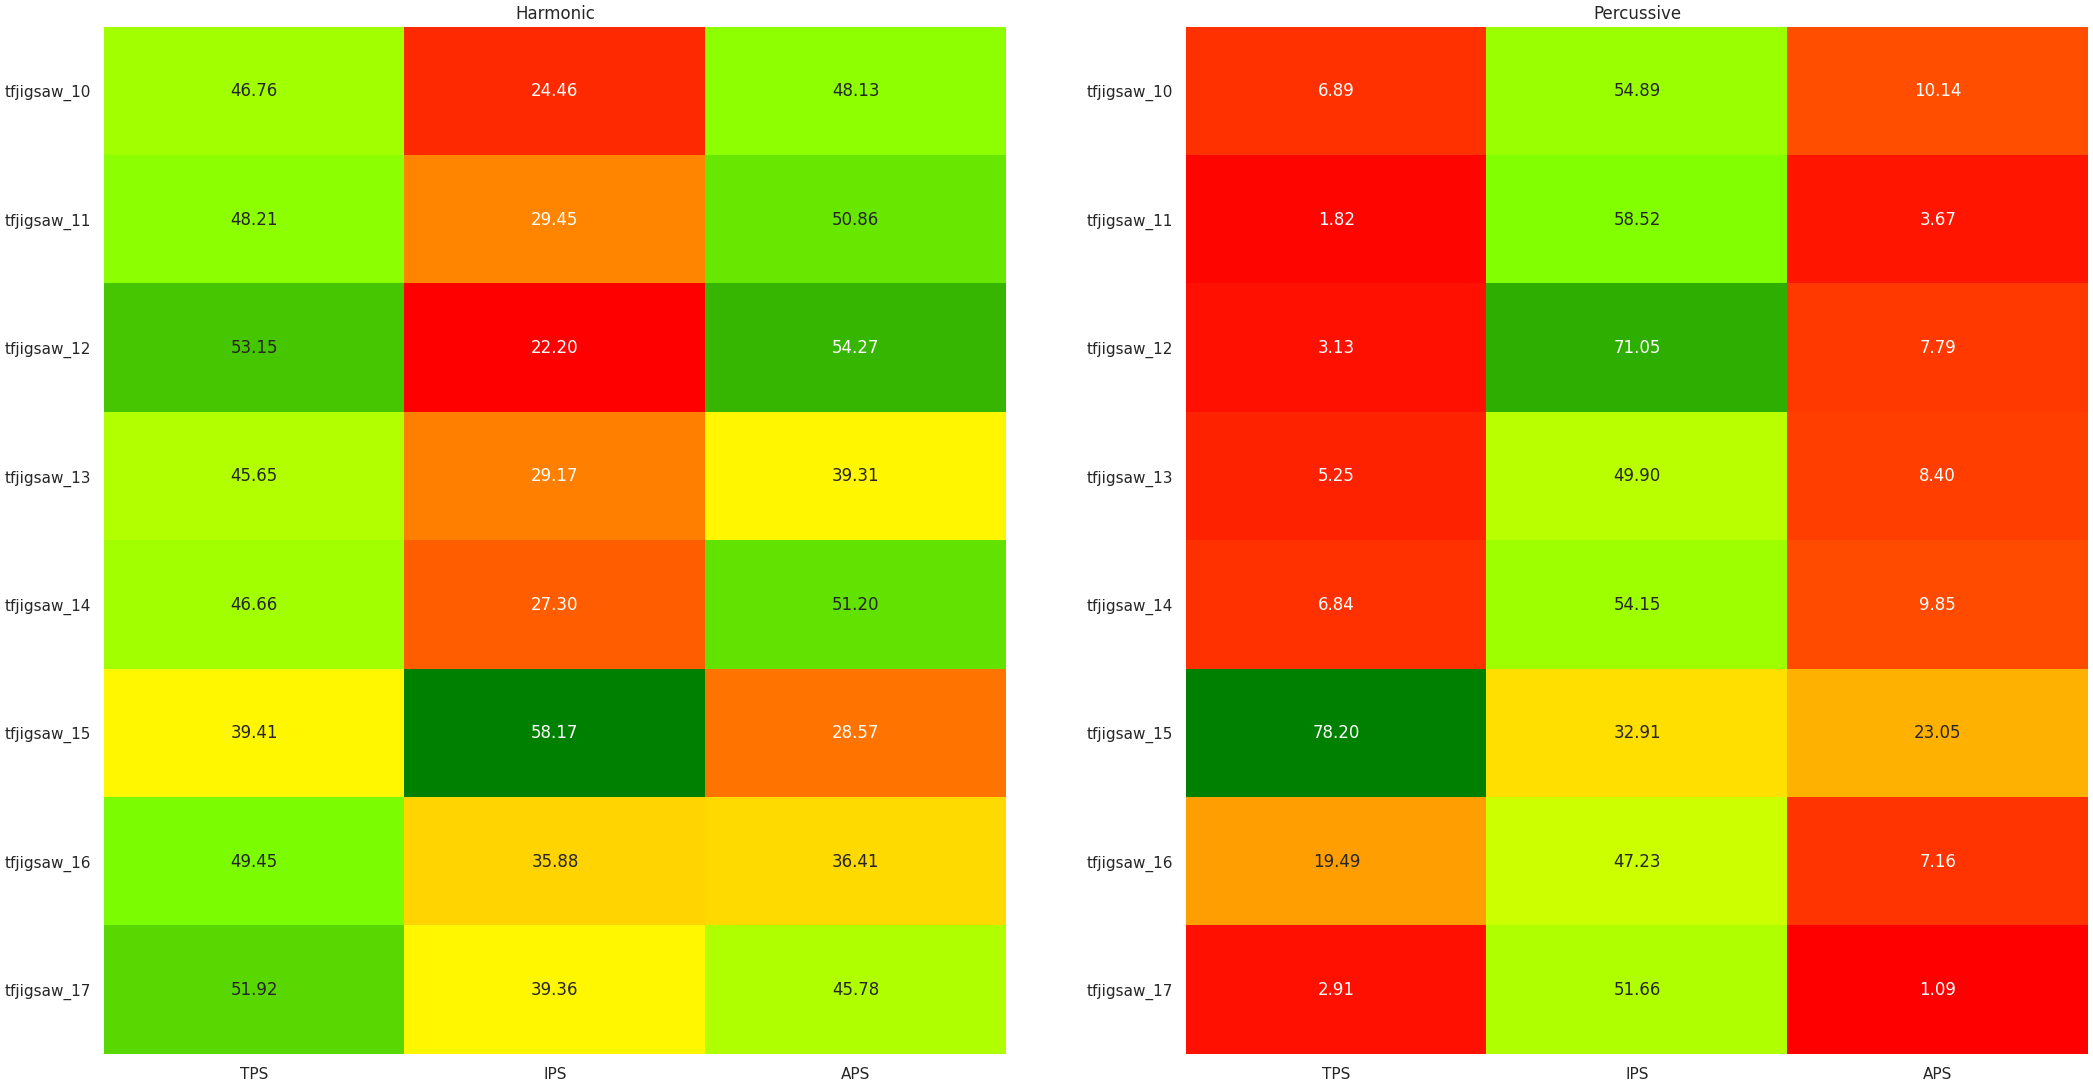
\includegraphics[width=16cm]{../evaluation/heatmaps/Jigsaw2_PEASS_abbrev.png}}
	\caption{TFJigsaw PEASS results}
	\label{fig:jigsaw}
\end{figure}

\vfill
\clearpage

\subsubsection{\textbf{\textcolor{red}{TODO }}WMDCTLasso}

\begin{figure}[ht]
	\centering
	\makebox[\textwidth]{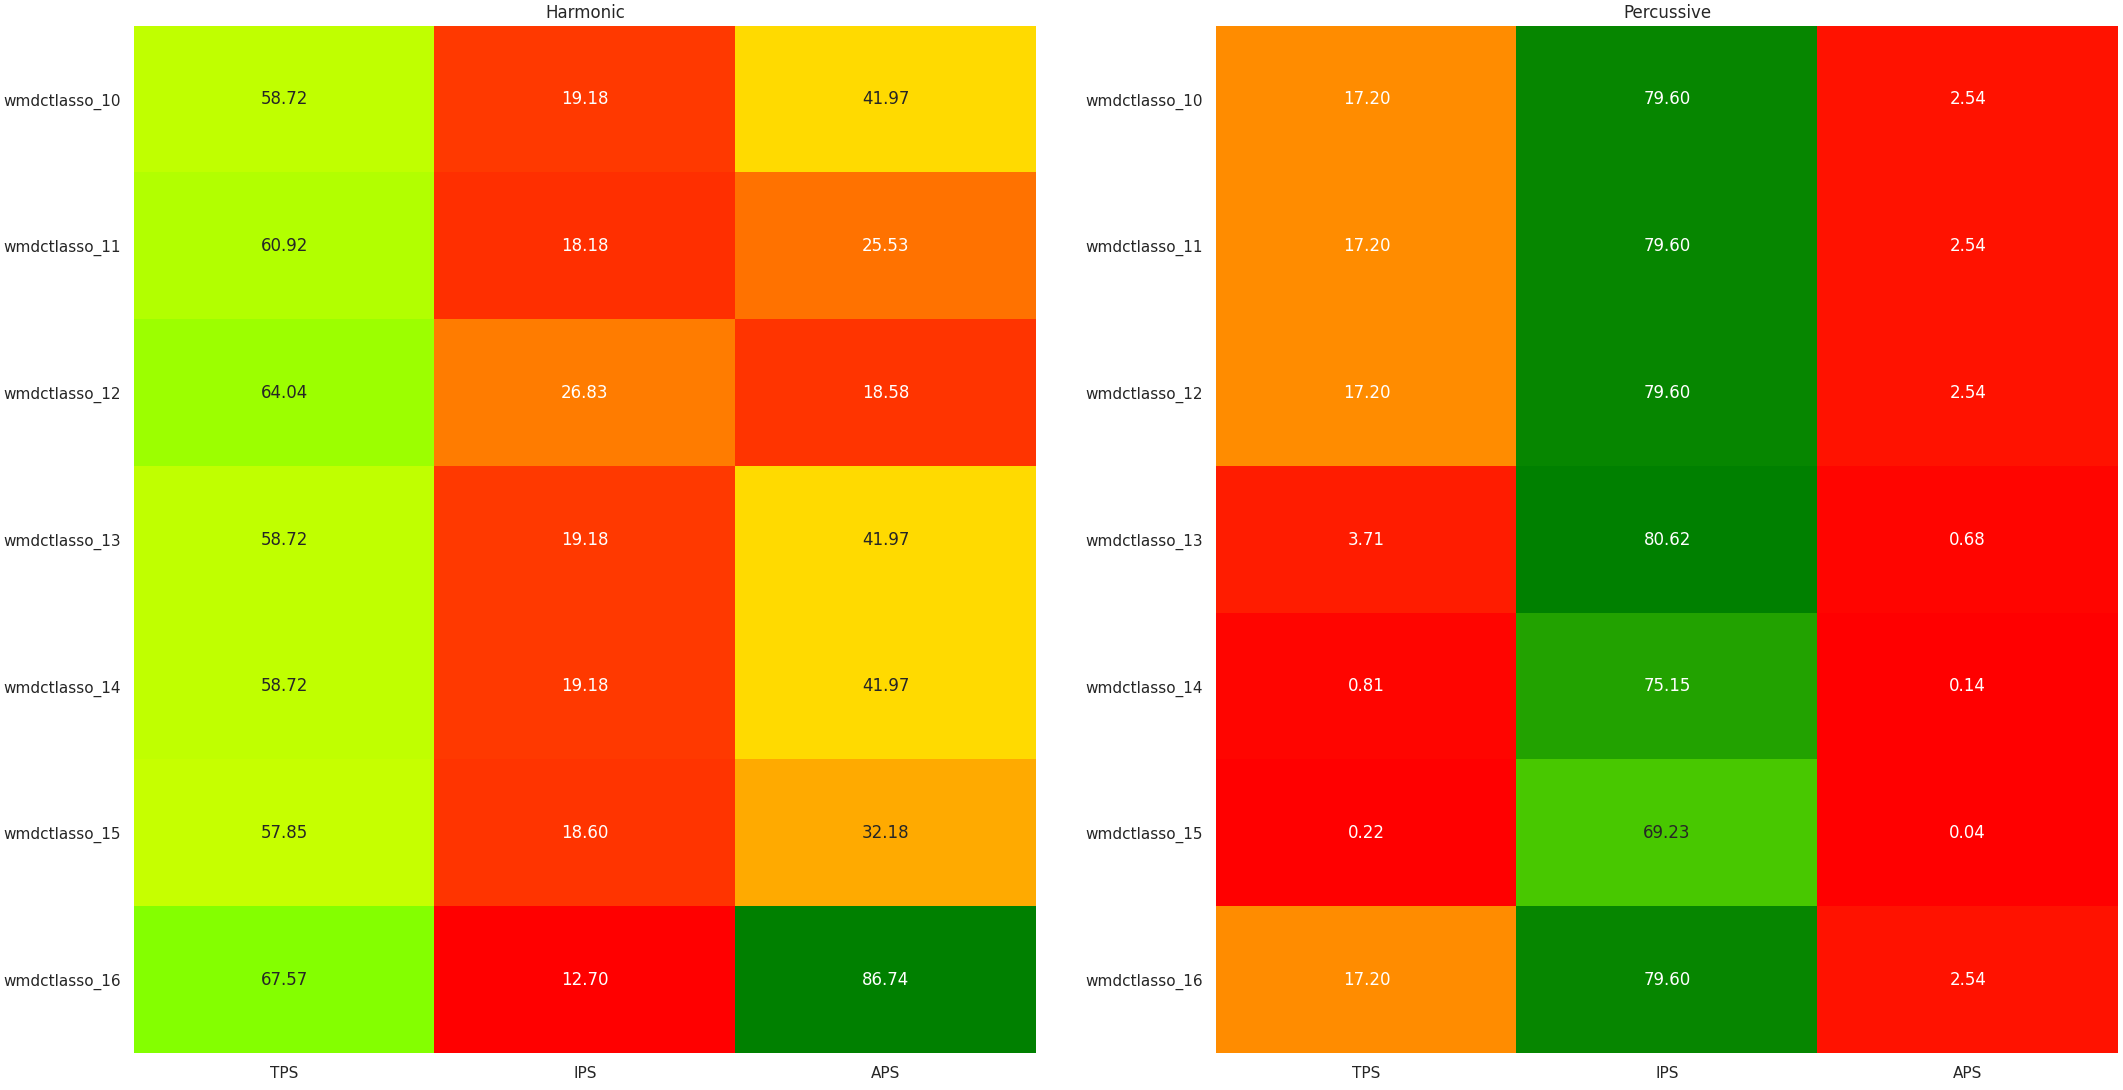
\includegraphics[width=16cm]{../evaluation/heatmaps/WMDCT2_PEASS_abbrev.png}}
	\makebox[\textwidth]{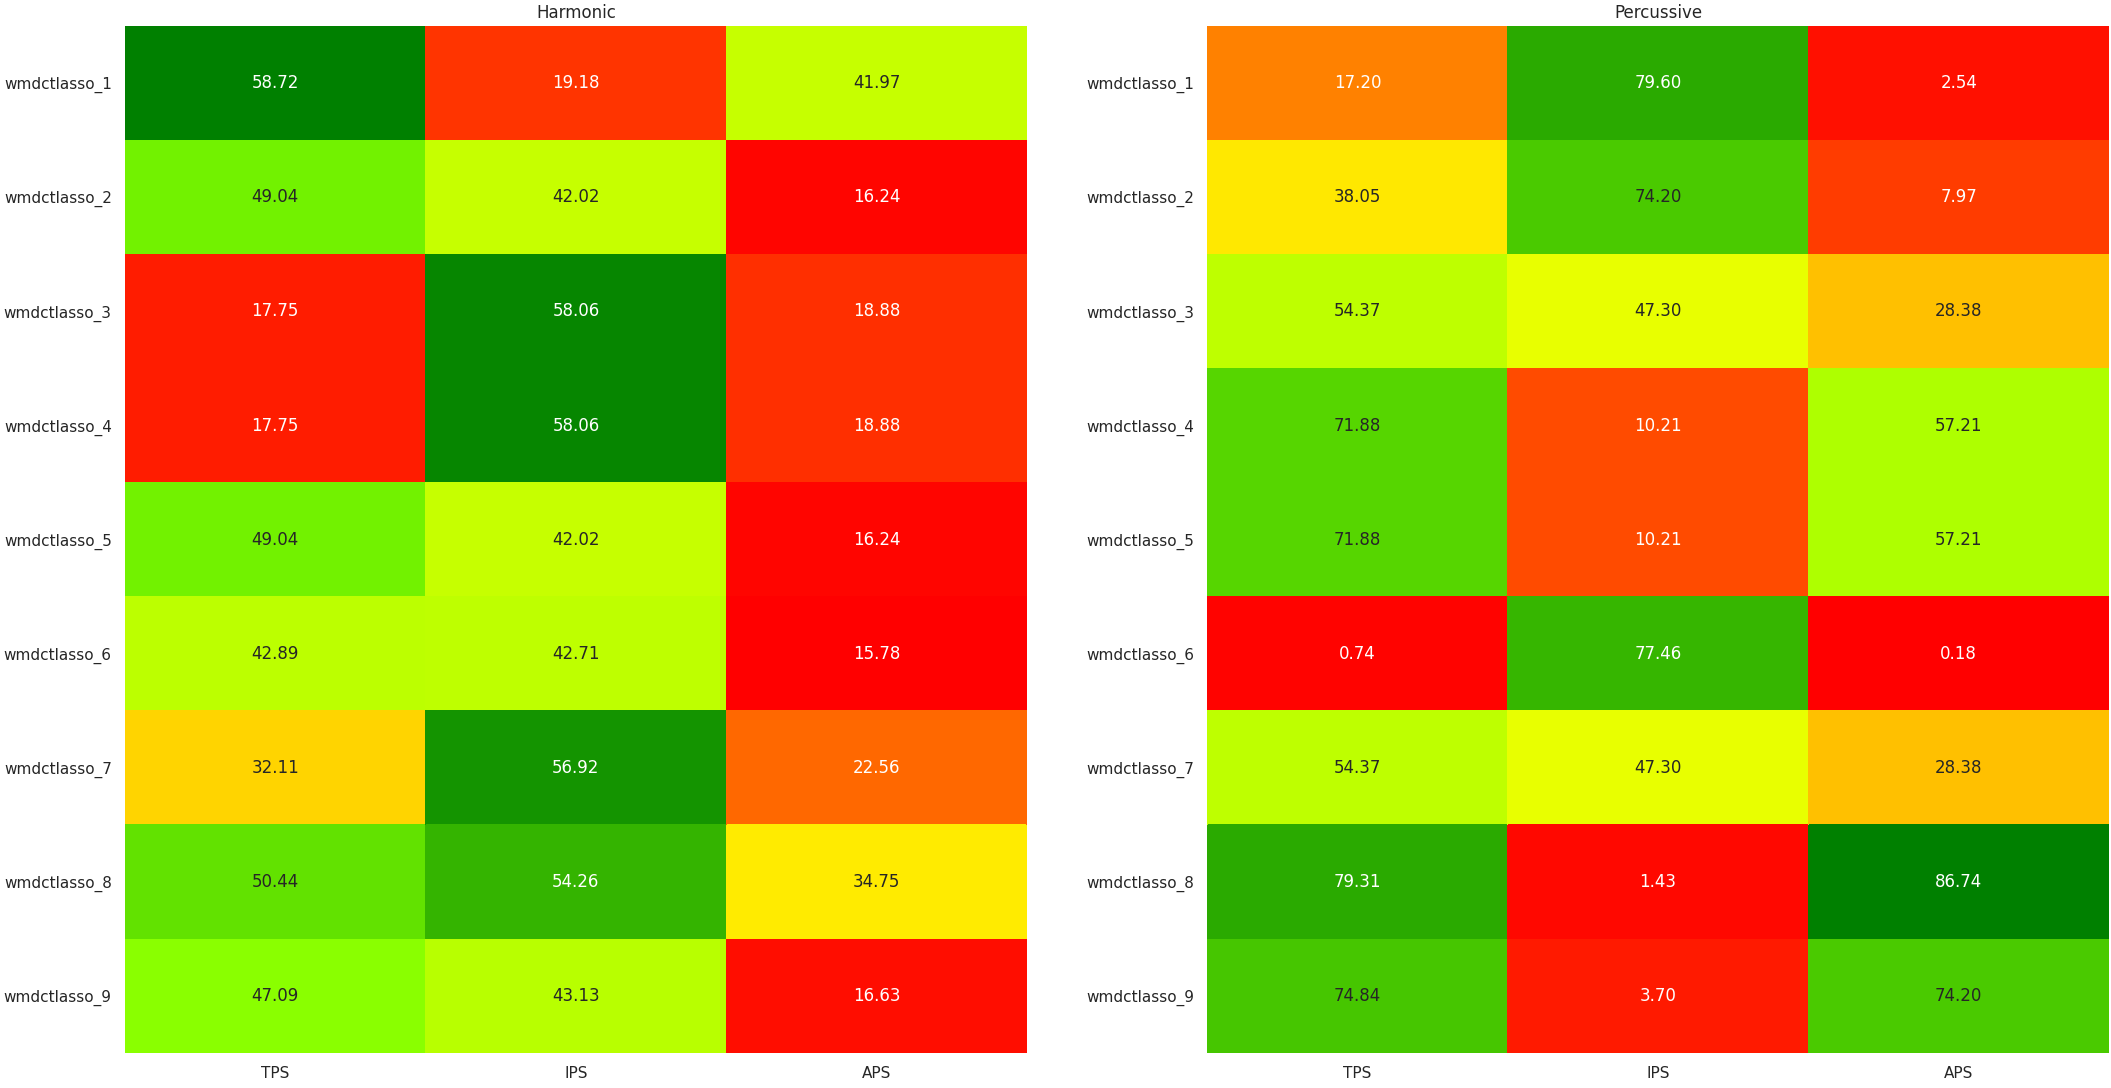
\includegraphics[width=16cm]{../evaluation/heatmaps/WMDCT_PEASS_abbrev.png}}
	\caption{WMDCT PEASS results}
	\label{fig:wmdct}
\end{figure}

\vfill
\clearpage

\subsubsection{Hybrid -- TFJigsaw-HPSS}

\begin{wrapfigure}{r}{5cm}
	\vspace{-1.0em}
	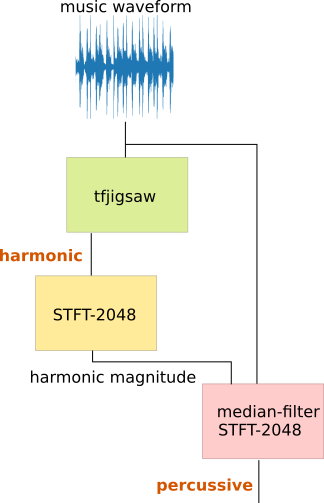
\includegraphics[width=5cm]{./hybrid_hpss_block_diagram.png}
	\caption{Hybrid HPSS}
	\label{fig:hybridhpss}
\end{wrapfigure}

The first hybrid algorithm created is for harmonic/percussive source separation. Noting that the \Verb#tfjigsaw-1# configuration achieved the best harmonic separation, and that median-filtering and soft masking with STFT-2048 achieved the best percussive separation, the proposed hybrid is a combination of both. First, the harmonic component is separated using TFJigsaw (the percussive output is discarded).

Next, median filtering with STFT-2048 is applied on the input signal, with a twist -- the percussive estimate is computed like typical, with a median filter. However, the harmonic estimate is computed by taking the STFT-2048 magnitude of the harmonic component output by TFJigsaw. The harmonic estimate from median filtering the STFT is discarded.

Finally, soft masks are computed from the percussive and harmonic estimates and applied to the STFT to get the percussive component. The block diagram of the proposed system is presented in figure \ref{fig:hybridhpss}.

In figure \ref{fig:finalhpss}, we can see that the hybrid HPSS combines good harmonic and percussive separations from the two original algorithms, respectively. The PEASS scores show that it compares favorably with the Open-Unmix neural network solution. The vocal hybrid (which will be shown next) has better percussive separation performance across all scores, but slightly worse interference in the harmonic separation.

\begin{figure}[ht]
	\centering
	\makebox[\textwidth]{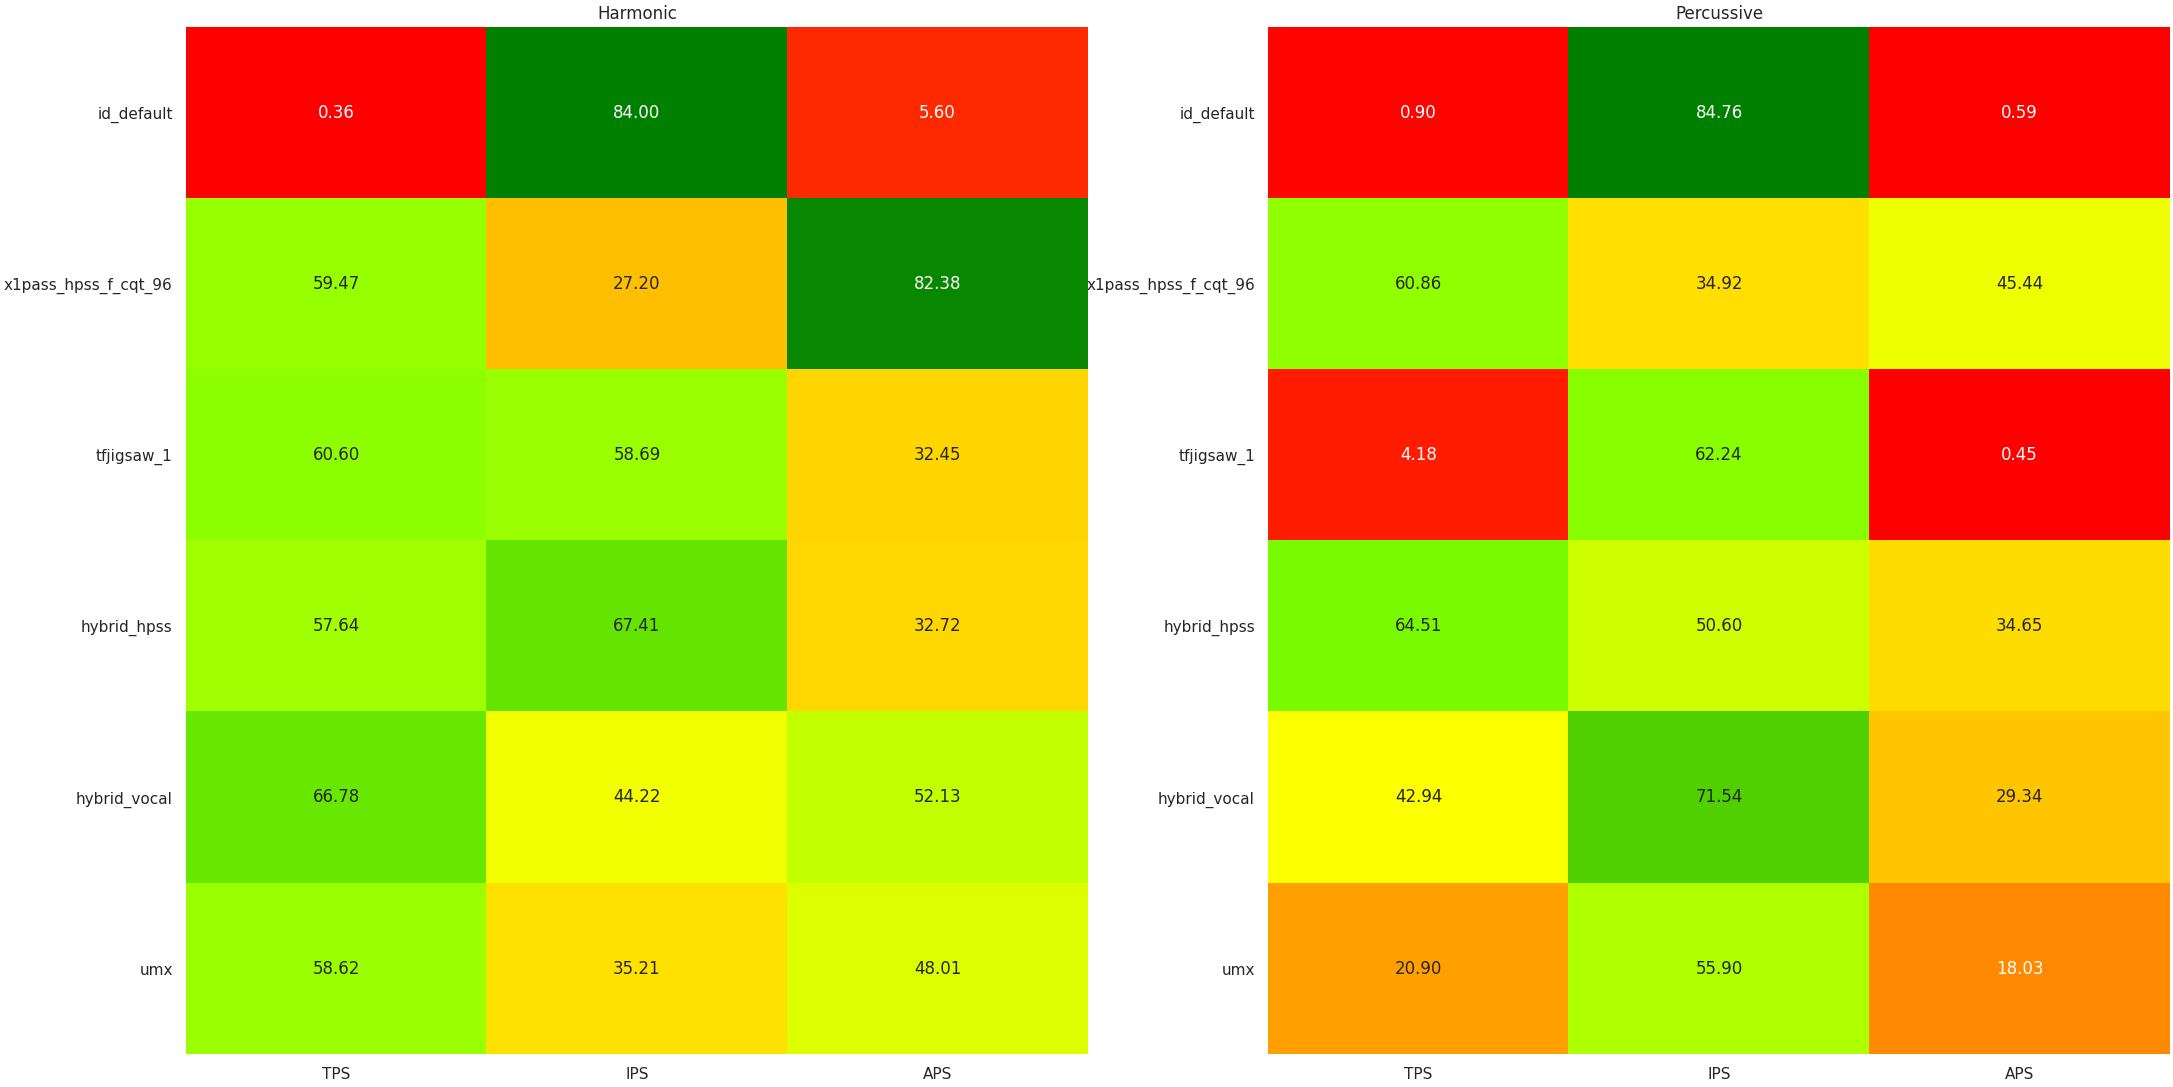
\includegraphics[width=16cm]{../evaluation/heatmaps/Final_HPSS_PEASS_abbrev.png}}
	\caption{Final HPSS results, PEASS scores}
	\label{fig:finalhpss}
\end{figure}

\subsection{Harmonic/percussive/vocal source separation}

The next task is harmonic/percussive/vocal source separation. The mixtures are combined from the instrument stems including vocals from the same 5 minutes of MUSDB18-HQ, and as before, the PEASS results are shown in heatmaps.

\subsubsection{Median-filtering with STFT/CQT masking}
\label{subsec:mfvocalsep}

The median filtering algorithms and a general framework for two-pass median filtering harmonic/percussive source separation were provided in \ref{subsec:mfilthpss}. The paper \cite{fitzgerald2} noted the following:
\begin{tight_enumerate}
	\item
		Using an STFT-16384 in the first pass led to a good harmonic separation
	\item
		Using an STFT-1024 in the second pass led to a good percussive separation
	\item
		Using a CQT-24 in the second pass led to a good vocal separation
\end{tight_enumerate}

The results are shown in figure \ref{fig:vocalround1soft}, and the algorithm names and configurations are described in table \ref{table:round3softvocal}. One interesting outcome is that using a CQT-96 in the first iteration in place of the STFT-16384 resulted in a better vocal and percussive separation, at the expense of the harmonic separation. The paper's original results were reproduced -- the variant with two linear STFTs (STFT-16384, STFT-1024) produced a better percussive and worse vocal separation, and the variant with a linear STFT and nonlinear CQT (STFT-16384, CQT-24) produced a better vocal separation.

\begin{table}[ht]
	\centering
\begin{tabular}{ |l|l|l|c|c|c| }
	 \hline
	  Name & First pass & Second pass  \\
	 \hline
	 \hline
	 mf\_default\_linear & STFT-16384 & STFT-1024 \\
	 \hline
	 mf\_default\_cqt & STFT-16384 & CQT-24 \\
	 \hline
	 mf\_cqt1 & CQT-96 & STFT-1024 \\
	 \hline
	 mf\_cqt2\_\{12-96\} & STFT-16384 & CQT-\{12-96\} \\
	 \hline
	 mf\_cqt3\_\{12-96\} & CQT-96 & CQT-\{12-96\} \\
	 \hline
\end{tabular}
	\caption{Multipass Fitzgerald configurations}
	\label{table:round3softvocal}
\end{table}

The CQT in the first position chosen is always the CQT-96, for maximum frequency resolution. The vocal separation has a stable quality in every case where the second pass is a CQT, regardless of the values for bins-per-octave. The percussive separation is best with a linear STFT-1024 in the second pass, but respectable with the CQT up to 48 bins-per-octave.

When choosing between the harmonic separation scores of the linear STFT-16384 and nonlinear CQT-96 in the first pass, we can see that using a CQT gives a very high target and artifact score, but a very poor interference score. In other words, there is hardly any separation being done. On the other hand, the target score of STFT-16384's harmonic separation is very low, indicating the absence of the desired sound.

\vfill
\clearpage % force a page break before references

\subsubsection{Hybrid -- Iterative-CQT-Sep}

\begin{wrapfigure}{r}{8cm}
	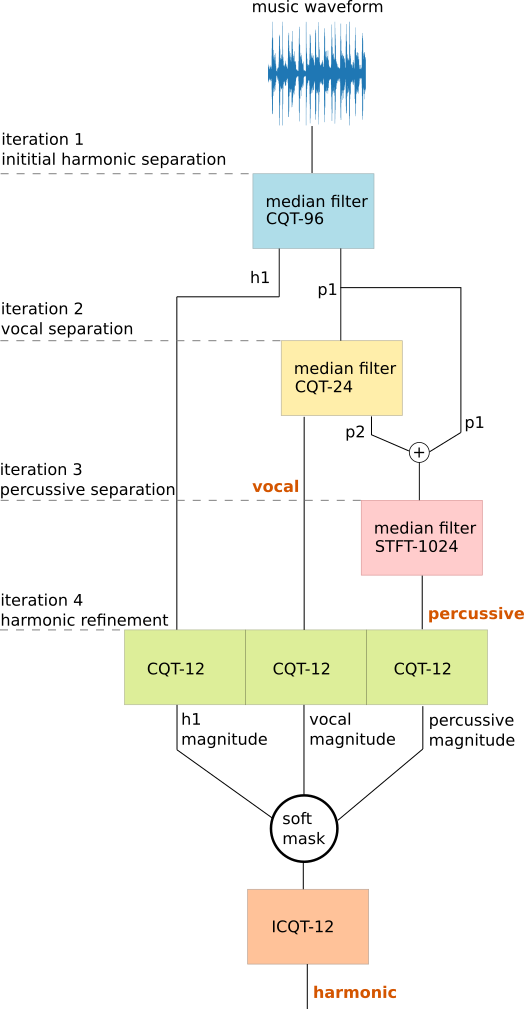
\includegraphics[width=8cm]{./hybrid_vocal_block_diagram.png}
	\caption{Hybrid harmonic/percussive/vocal block diagram}
	\label{fig:hybridvocal}
\end{wrapfigure}

In section \ref{subsec:mfvocalsep}, \citet{fitzgerald2}'s multipass algorithm for harmonic/percussive/source separation was presented and evaluated. The authors' findings were confirmed -- following a first iteration for harmonic separation with an STFT-16384, using a CQT-24 in the second iteration gives a good vocal estimate, and using an STFT-1024 in the second gives a good percussive estimate. It was also noted that using the CQT-96 in the first iteration led to a higher quality percussive or vocal separation in the next iteration, but created a high-interference harmonic separation. The hybrid combines all of the above findings with some refinements:

\begin{tight_enumerate}
	\item
		Median-filter CQT-96 in the first position -- the harmonic output is the ``almost final'' harmonic component, and the percussive output is the next input.
	\item
		Median-filter CQT-24 in the second iteration, where the harmonic output is the final vocal component. Add the percussive separation from this iteration to the percussive output of previous iteration, to use as the next input.
	\item
		Median-filter STFT-1024 in the third, where the percussive output is the final percussive component.
	\item
		Using a CQT-12, get harmonic, vocal, and percussive magnitude estimates from the ``almost final'' harmonic and final vocal and percussive components. Create and apply a soft mask for harmonic refinement, in an attempt to reduce vocal and percussive interference.
\end{tight_enumerate}

The system is shown in the block diagram in figure \ref{fig:hybridvocal}.

The results of the evaluation are in figure \ref{fig:finalvocal}. The hybrid vocal algorithm gets the best percussive score, beating the multipass Fitzgerald configuration from the paper\cite{fitzgerald2} which had the highest percussive score. The harmonic score sacrifices interference for a better target and artifact scores. However, note that the interference score (16.32) is higher than the original interference score of the CQT-96 in the first position (4.81). This shows that the fourth step for harmonic refinement had the desired effect of reducing the interference in the harmonic separation.

\begin{figure}[ht]
	\centering
	\makebox[\textwidth]{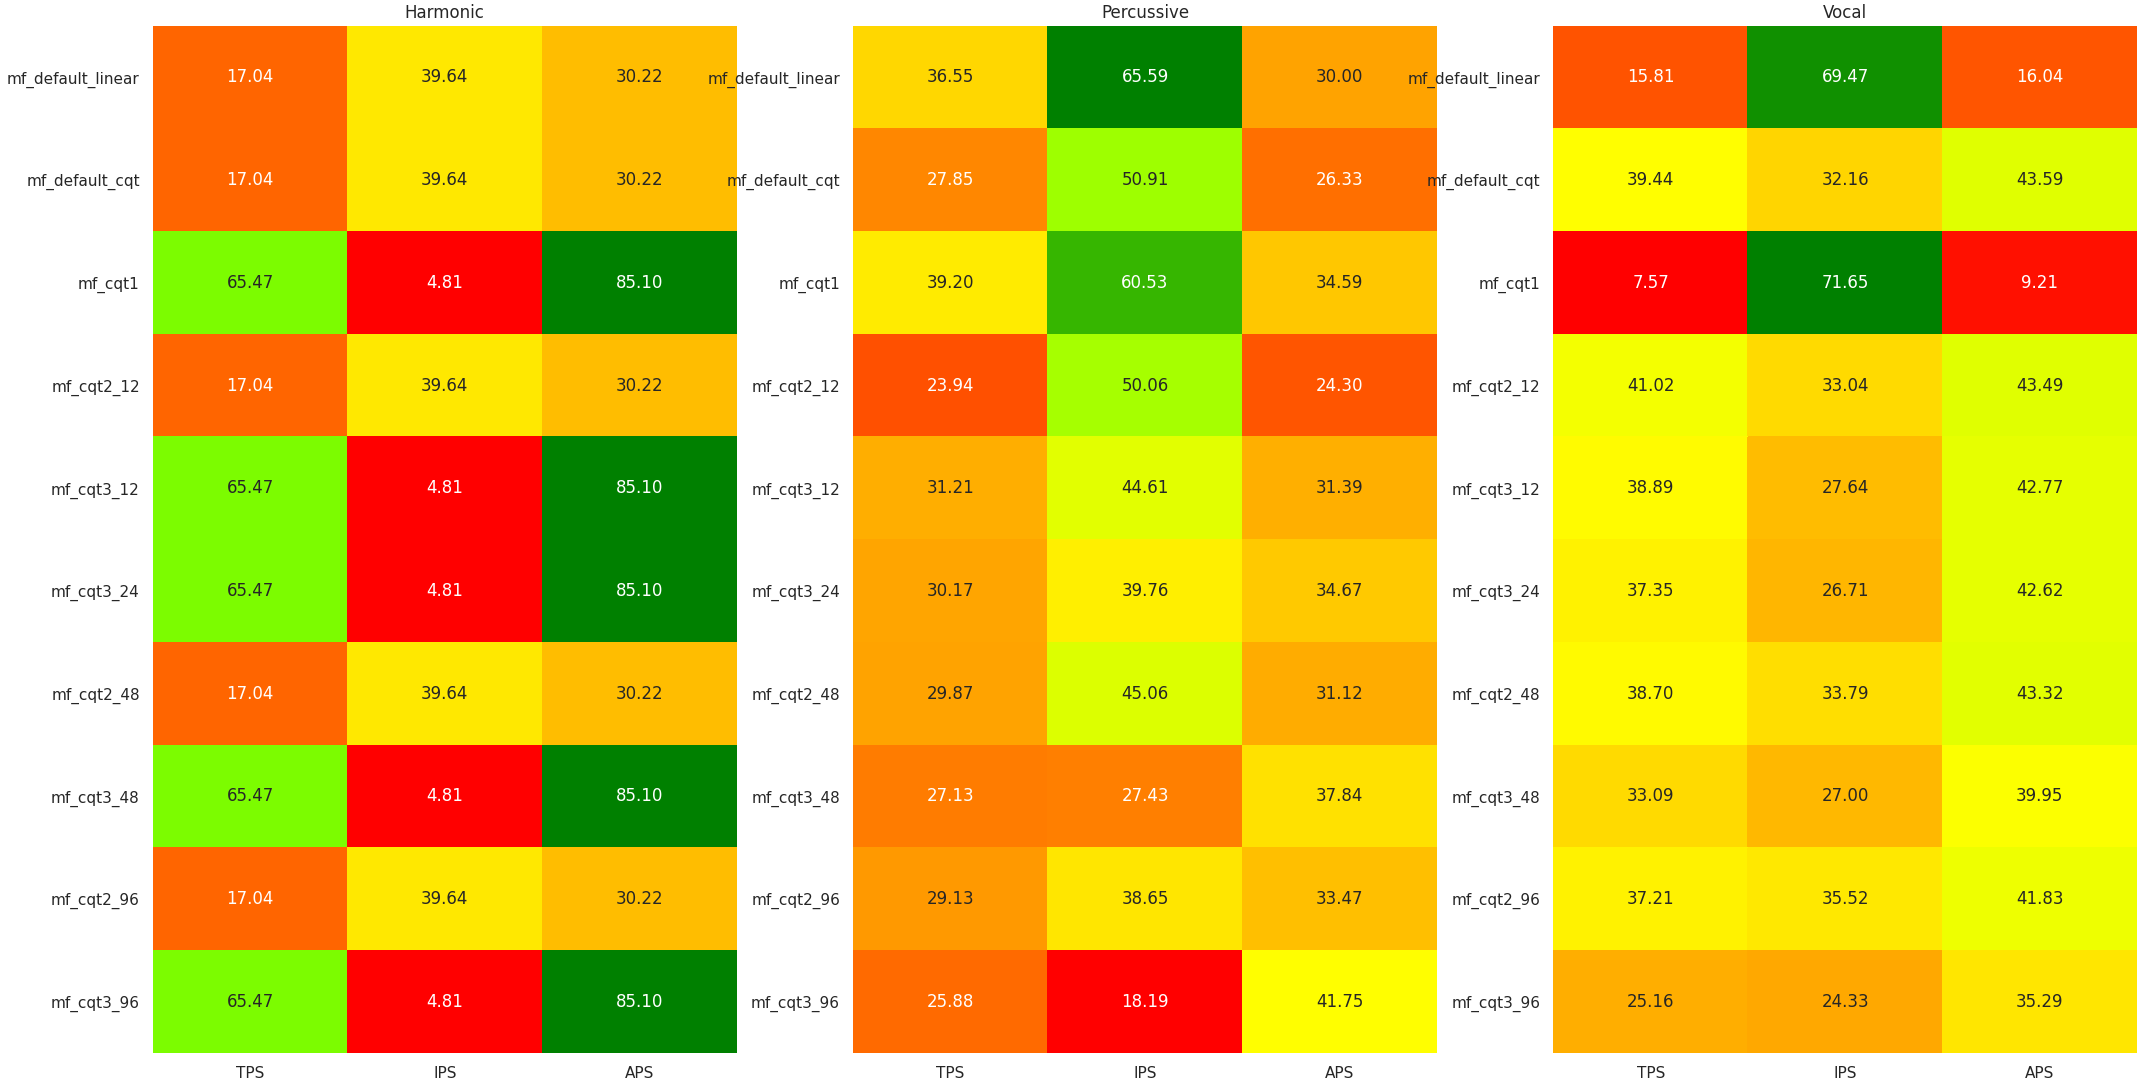
\includegraphics[width=16cm]{../evaluation/heatmaps/2pass_Fitzgerald_PEASS_abbrev.png}}
	\caption{Multipass Fitzgerald (soft mask) PEASS results}
	\label{fig:vocalround1soft}
	\vspace{1em}
	\makebox[\textwidth]{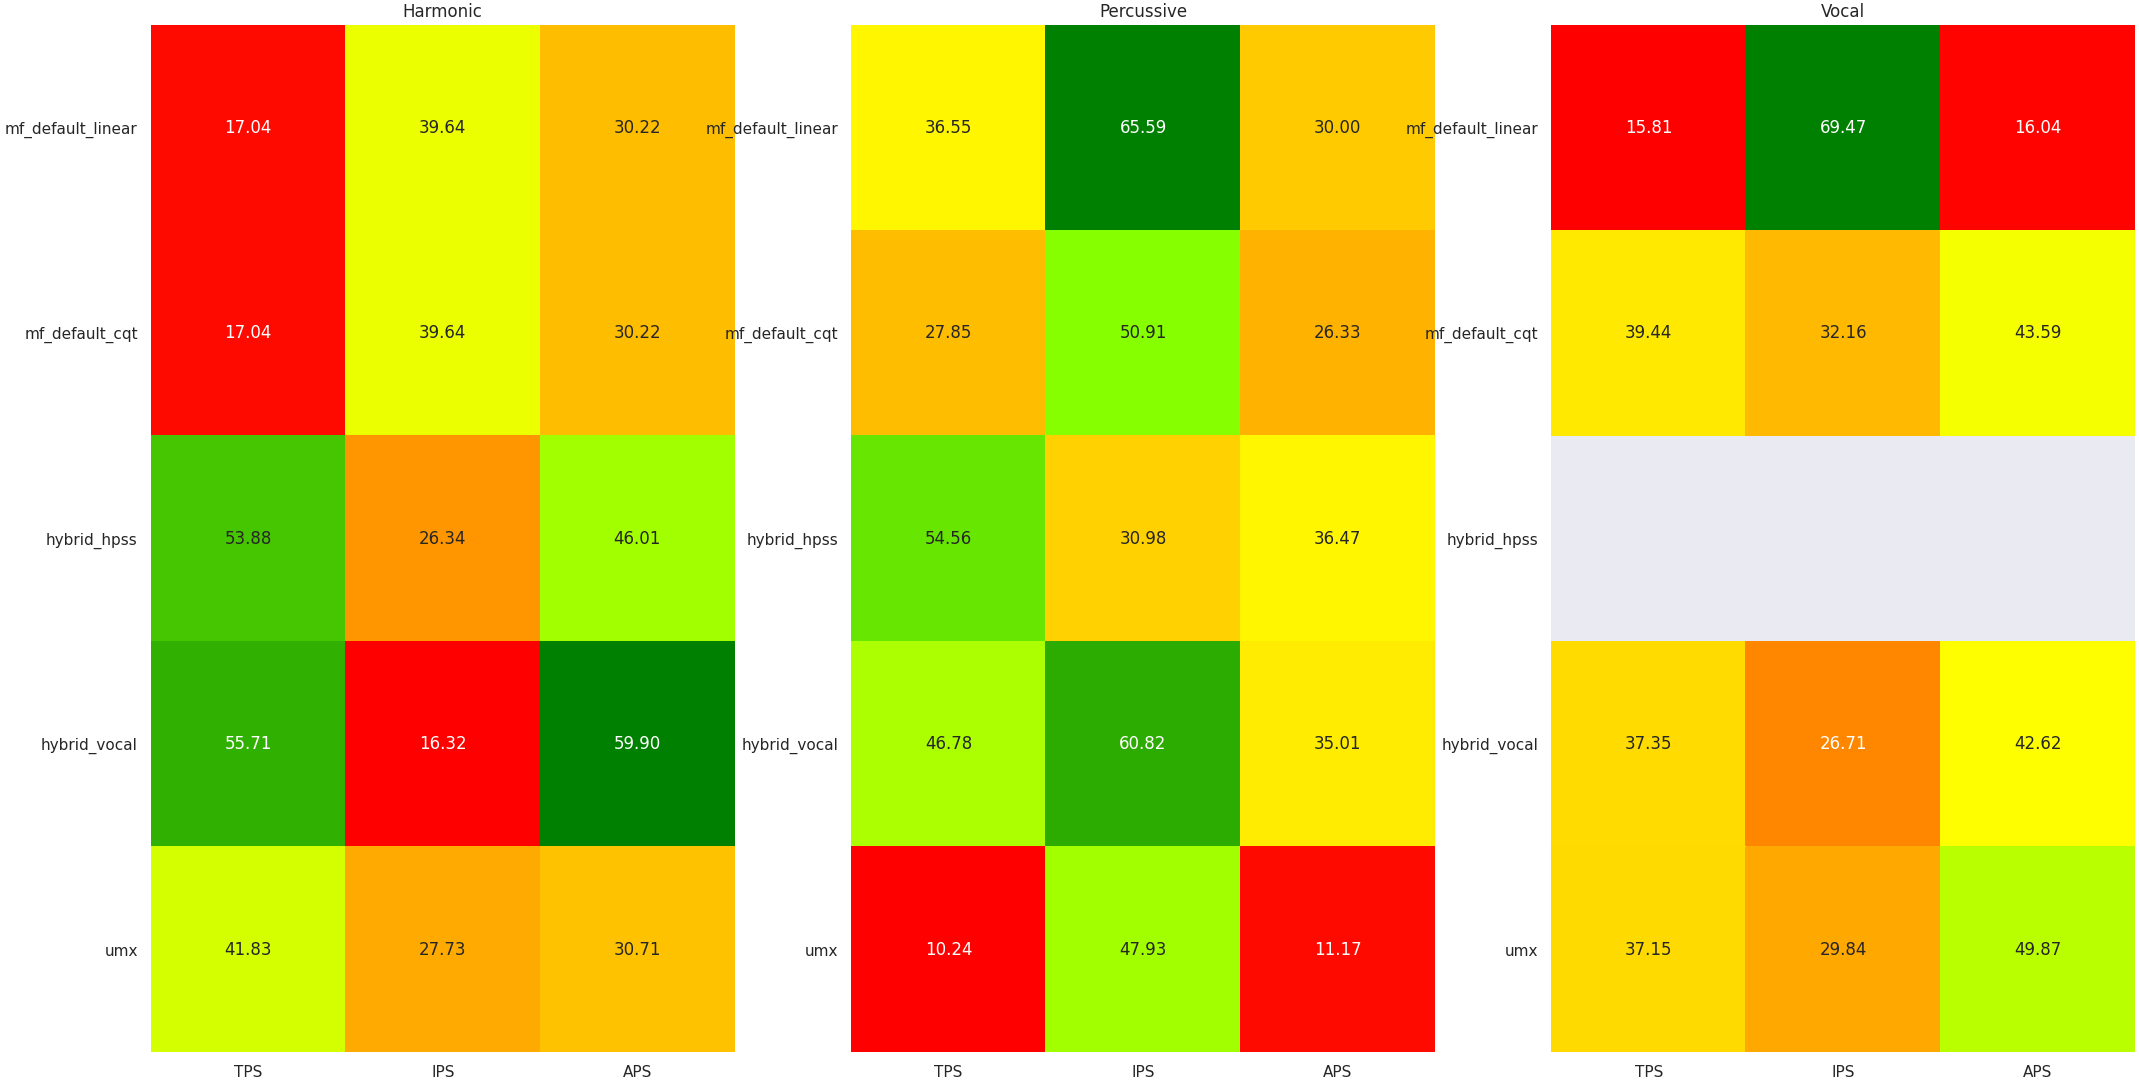
\includegraphics[width=16cm]{../evaluation/heatmaps/Final_Vocal_PEASS_abbrev.png}}
	\caption{Final vocal results, PEASS scores}
	\label{fig:finalvocal}
\end{figure}

\vfill
\clearpage % force a page break before references

\section{\textbf{\textcolor{red}{TODO }}Discussion and conclusion}

The first thing I will mention is that despite showing good PEASS scores, the conclusion is not certain that the presented hybrid algorithms beat a state-of-the-art neural network. The neural network has been trained and evaluated with BSS, an alternative 

\vfill
\clearpage % force a page break before references

%\nocite{*}
\printbibheading[title={References}]
\printbibliography[heading=none]

\end{document}
